\documentclass[12pt]{article}
\usepackage[utf8]{inputenc}%encodage des caractères
\usepackage[T1]{fontenc}%encodage de la police
\usepackage[frenchb]{babel}%langue française
\usepackage{tikz}
\usetikzlibrary{arrows,decorations.pathmorphing,backgrounds,positioning,fit,matrix}
\usepackage{listings}
\usepackage[linesnumbered,ruled]{algorithm2e}%linesnumbered permet de numeroter les lignes, ruled permet un affichage avec des lignes separatrices
\usepackage[a4paper,left=2cm,right=2cm,top=2cm,bottom=2cm]{geometry}
\usepackage{hyperref}
\setlength{\parindent}{0cm}
\setlength{\parskip}{1ex plus 0.5ex minus 0.2ex}
\newcommand{\hsp}{\hspace{20pt}}
\newcommand{\HRule}{\rule{\linewidth}{0.5mm}}
% Titre
\title{Structure du projet de moteur 3D}
\date{}%no date
\begin{document}
\begin{titlepage}
  \begin{sffamily}
  \begin{center}
    % Upper part of the page. The '~' is needed because \\
    % only works if a paragraph has started.
    \textsc{\LARGE Université de Caen}\\[2cm]
    \textsc{\Large Rapport Conception logicielle avancée}\\[1.5cm]
    % Title
    \HRule \\[0.4cm]
    { \huge \bfseries RAPPORT DU PROJET DE RENDU 3D PAR LANCER DE RAYONS
 \\[0.4cm] }
    \HRule \\[1cm]
    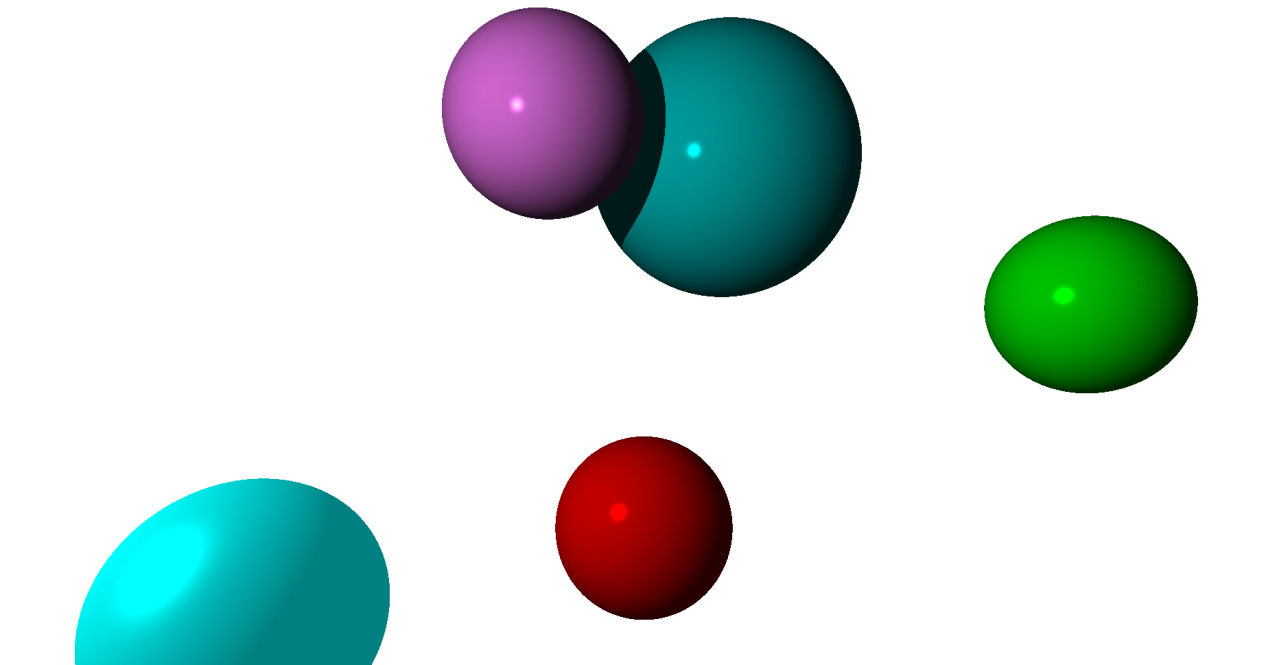
\includegraphics[scale=0.3]{./images/pic1.png}
    \\[1cm]
    % Author and supervisor
    \begin{minipage}{0.7\textwidth}
      \begin{flushleft} \large
        ABBAD KAMEL - 21911536 \\
        BOUSADIA LAHCENE - 21911132 \\
        MARTIN MAXENCE - 21807030\\
 		MEYER ARTHUR - 21805134 \\
      \end{flushleft}
    \end{minipage}
    
    \begin{minipage}{0.4\textwidth}
    \end{minipage}
    \vfill
    \HRule \\[0.4cm]
             PROFESSEUR : G. Bonnet, C. Alec \\
             {\large 07 April 2020}
    \HRule \\[0.4cm]
  \end{center}
  \end{sffamily}
\end{titlepage}
    \newpage	
	\begin{center}
		\tableofcontents
	\end{center}
	\section{Présentation du projet}
	\subsection{Spécification minimal demandé}
	    Le ray tracing (lancé de rayons) est un moyen de visualisation des modèles 3D, pour pouvoir créer des effets spéciaux, créer des images gérant des éclairages,la réflection ...
	    
	    L'objectif de notre project est de faire une application qui prend un fichier décrivant une scène au format ".pov" et de créer l'image associé. Pour pouvoir afficher l'image on doit lire le fichier qui décris la scène puis y appliquer un lancé de rayons pour créer une image où chaque rayons est un pixel qui change de couleurs en fonction de l'acteur touché, de l'éclairage etc ... Pour ce faire nous devions utiliser un peu d' algèbre et de géométrie pour colorer correctement rayons (et donc pixels).
	    
	    On peut donc résumer les principales étapes a réaliser comme ceci :
	    
            \begin{enumerate}
                \item Lire le fichier (.pov).
                \item Créer la scène
                \item Lancer les Rayons
                \item Afficher l'image
            \end{enumerate}
    \subsection{Fonctionnalités implémentés}
        Dans notre programme nous avons implémenté plusieurs fonctionnalités. Certaines demandés, d'autres en complement pour une meilleurs ergonomie. Nous avons 4 fonctionnalités nécessaires :
        
        \begin{enumerate}
            \item Lecture du fichier ".pov".
            \item Création de la scène a partir du fichier.
            \item Applications des effets d'éclairages (lancé des rayons).
            \item Affichage de l'image finale.
        \end{enumerate}
        
        A lesquels s'ajoute 4 autres fonctionnalités pour une meilleur ergonomie de l'application :
        
            \begin{itemize}
                \item Possibilité de charger une scène sans avoir a relancé l'application
                \item Possibilité de créer une scène de 0 ou d'en modifier une
                \item Possibilité de sauvegarder une scène
                \item Possibilité de se déplacer dans la scène
            \end{itemize}
            
        Grâce a ces fonctionnalités nous avons une application fonctionnel et plutôt simple et intuitive d'utilisation pour l'utilisateur.
        \subsection{Librairies utilisés}
            Dans ce projet nous avons utilisé différentes librairies qui sont: 
            
                \begin{enumerate}
                    \item "Swing" ( JPanel, JFrame, JScrollPane ...)
                    \item "AWT" ( Dimension, Toolkit, BorderLayout ...)
                    \item "Util"
                \end{enumerate}
        \paragraph{}
        Swing un outils de widget d'interface utilisateur graphique qui permets la création de fenêtres : JFrame, JPanel par exemples. C'est cette librairie que nous mettons en page les divers éléments de l'application.\\
        AWT est une librairie de contrôles intégrés tels que des boutons, des barres d'outils, des sélecteurs de paramètre,et des zones de texte pour afficher ou pour saisir des données.\\
        "Util" est une libraires de class facilitant le développement, la class que nous utilisons le plus est ArrayList qui sert pour créer des liste d'objets.
        		
\section{Organisation du projet}
		\subsection{Arborescence des packages}
		       \paragraph{}
		       Dans notre projet on a crée un grand dossier <<Engine>> qui est le principal package qui est constitué de trois autres répertoires aussi.
		       
		       \begin{figure}[h]
                    \begin{center}
                    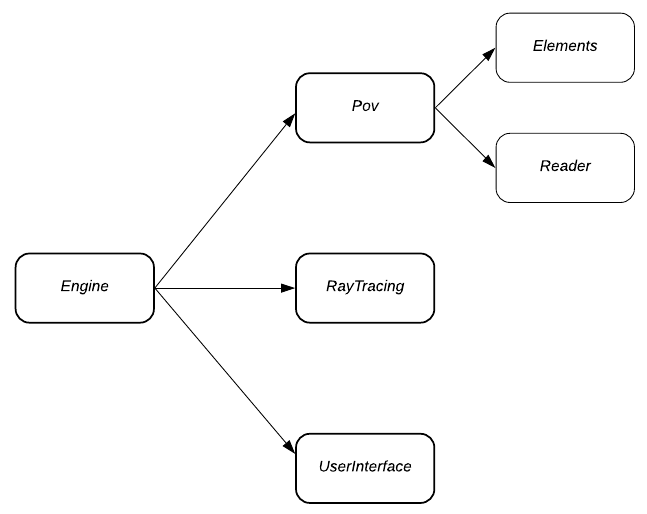
\includegraphics[width=0.5\textwidth]{./images/Arborescence.png}
                    \end{center}
                    \caption{Arborescence des packages.}
                    \label{fig}
                \end{figure}
		       
		       \paragraph{}
		       Le premier package est POV qui se divise en deux packages <<Elements>> et <<Reader>>, dans le répertoire Éléments on trouve toutes les classes qui sont responsable des acteurs(formes géométriques), caméra et la lumière. Reader est le package qui représente tout ce qui est chargement, sauvegarde et création des scènes ou on trouve les classes Creator,Parser,Loader...
		       
		       RayTracing est le deuxieme package qui contient deux principales classes <<Ray>> et <<Vector>> c'est à dire toutes les classes qui gèrent les rayons et toutes les equations des vecteurs qui y sont associés. On peut dire que ce package est important pour notre projet.
		       
		       Troisièmement on trouve le package UserInterface qui est responsable de l'afffichage d'interface graphique (bouttons de sauvegarde, update, vue...), il contient aussi la classe exécutable Main.
		\newpage
		\subsection{Diagramme de classe}
		\paragraph{}Afin de simplifier notre code, on a crée deux diagrammes de classe qui présentent les classes et les interfaces du projet ainsi que les différentes relations entre celles-ci, les voici :
		
			\subsubsection{Core}
			\paragraph{}UML des classes du Core\footnote{toutes le classes qui ne concerne pas l'interface graphique}
			    \begin{figure}[h]
                    \begin{center}
                    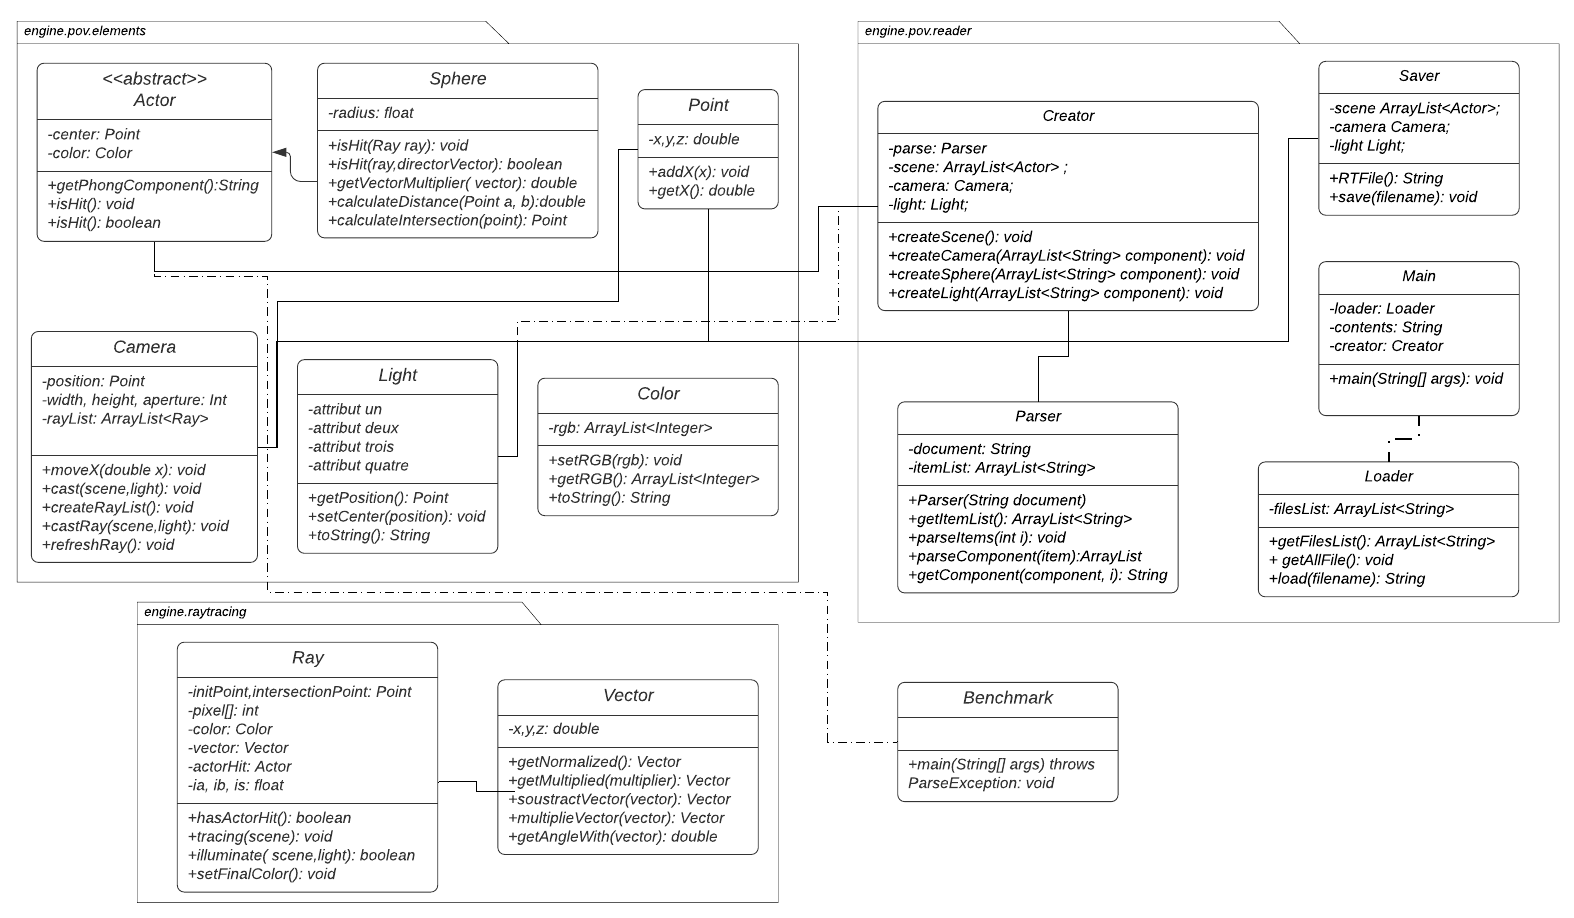
\includegraphics[width=1.1\textwidth]{./images/Core.png}
                    \end{center}
                    \caption{UML du Core.}
                    \label{fig}
                \end{figure}
            \newpage
			\subsubsection{Interface}
			\paragraph{}UML pour les classes en rapport avec l'interface graphique.
			    \begin{figure}[h]
                    \begin{center}
                    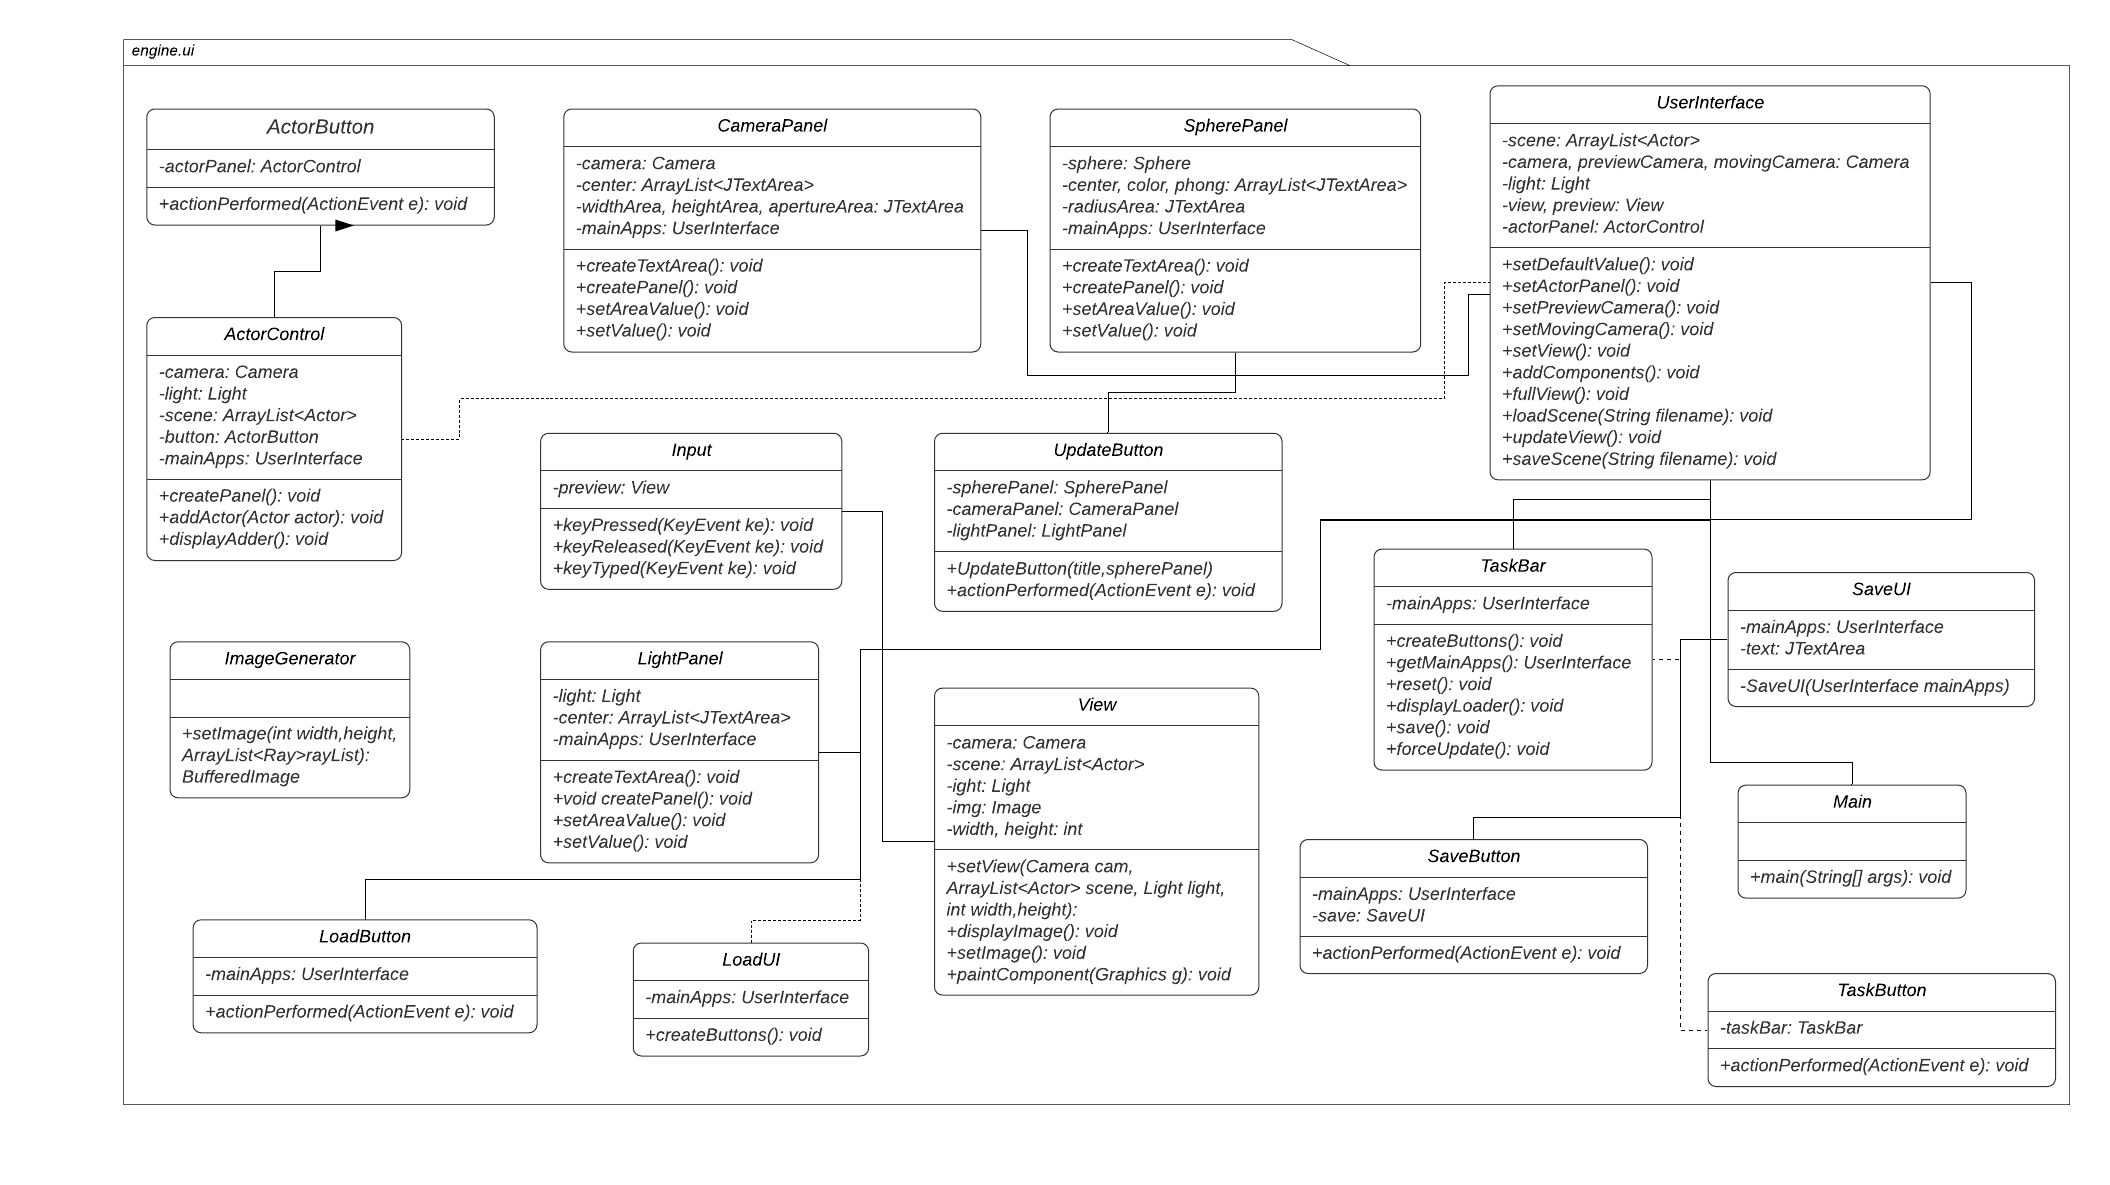
\includegraphics[width=1.1\textwidth]{./images/Interface.png}
                    \end{center}
                    \caption{UML de l'interface.}
                    \label{fig}
                \end{figure}
		\subsection{Répartition des tâches}
		Le projet a été divisé sur 4 principales taches ou chaque membre du groupe a son travail:
		\begin{figure}[h]
        	\begin{center}
            	\begin{tabular}{|c|c|}
			\hline
			\textbf{MEMBRE} & \textbf{TACHE}\\
  			\hline
 			Arthur & Lecture du fichier pov et création de la scène\\
  			\hline
  			Kamel & Affichage de la scène (création de l'image suivant les "rayons")\\
  			\hline
  			Lahcene & Création de toutes les classes d'objets et diaporama\\
  			\hline
  			Maxence & Gestion du lancé de rayons\\
  			\hline
		\end{tabular}
        \end{center}
        \caption{Tableau de répartition des taches.}
        \label{fig}
        \end{figure}
		\paragraph{}Pour le rapport chaque membre a pris une partie pour qu'on facilite le travail du groupe.
	\newpage
	
	\section{Problèmes et solutions}
		\subsection{Camera}
			\subsubsection{Lancement des rayons}
				\paragraph{Création des rayons}
				La création des rayons a été le premier problème qui s'est posé a nous. Il s'agit de la base du moteur 3D puisque c'est grâce a ces rayons que nous allions construire l'image final.
				
				Le problème était de partir d'un point de l'espace pour créer une image 2D, pour ce faire, grâce aux liens fourni dans l' énoncé, nous avons trouver qu'il fallait créer des rayon représenté par des vecteurs qui ont pour origine la caméra. Pour limiter les problèmes dû a une éventuelle rotation de la camera, nous avons décidé de ne pas implémenter la rotation de la camera dans un premier temps pour l'ajouter si il nous restais du temps une fois la majeur partie du projet fini. Donc les rayons ont des vecteurs de la forme ([-1;1];[-1:1];1).
				
				Il ne manquais plus qu'a trouver le moyen de savoir de quel couleur rayon devais être. Pour ce faire nous avons vérifié si il existais au moins 1 intersection entre un rayons et les acteurs, et si il en existais plusieurs, nous prenons le plus proche. Le rayon prenais alors la couleur de l'acteur touché a laquelle on applique l'ombrage de phong pour avoir un rendu réaliste.
				
				Ainsi en convertissant chaque rayons a un pixel de l'image grâce a sa couleur nous obtenons une image de la scène. 
				\paragraph{Échelle de l'image}
				L'échelle de l'image a posé un problème pour avoir des tailles différentes d'image, en effet au début, les vecteurs des rayon étaient générés de 1 a -1 sur l'axe X et sur l'axe Y. Ce qui fait que sur des définitions d'images autres que 1:1 l'image se retrouvait déformé malgré un nombres de pixels correct. Pour pallier a ce problème nous avons dû trouver le moyen de réduire la plage de valeur de Y pour coller a la définition de l'image. Pour ce faire si nous avons une image X:Y, alors Y doit varier de -Y/X a Y/X.
				
				Ainsi quelque soit la définition de l'image choisi, il n'y a aucune déformation.				
				\paragraph{Actualisation de l'image}
				Nous avons rencontré un soucis avec l'actualisation de l'image dans le cadre du déplacement de la camera : Les images se superposais. Après multiple tentative de correction du problème nous nous sommes rendu compte qu'en réalité le problème ne venais pas de l'interface mais du code. En effet nous réutilisions la fonction "castRay" qui permettais de lancer les rayons, sans réinitialiser les valeurs par défaut des rayons.
				
				Donc des rayons qui ne devais pas prendre de couleurs d'acteurs étais coloré car il gardais la couleur de l'acteur touché. En remettant les valeurs par défaut le problème a été résolu.
			\subsubsection{Déplacements}
			Pour le déplacement de la camera nous utilisons les KeyListener qui permettent d'écouter lorsqu'une touche du clavier est pressé. En redéfinissant la méthode "keyPressed" nous incrémentons les coordonnées de la camera suivant la touche actionnée : l'axe X de -1 pour la touche "q", +1 pour "d", l'axe Y de -1 pour "c", +1 pour "espace" et enfin l'axe Z de -1 pour la touche "s" et +1 pour la touche "z".
			
			Enfin nous actualisons l'image pour avoir la nouvelle vu depuis les nouveaux coordonnées de la camera.
		\subsection{Acteurs}
			\subsubsection{Intersection avec un rayon}
			Il nous a fallu définir une intersection entre les acteurs et les rayons. Pour se faire nous avons défini les méthodes abstraites "isHit" qui nous permettent ainsi grâce a une liste d'acteurs d'utiliser les méthodes "isHit" avec des manières de calculs différentes, car chaque forme a une fonction mathématique différente pour calculer l'intersection entre un vecteur et la dite forme. 
			
			Pour chaque forme on calcul les racines de l'équation du second degré associé a chaque plans de chaque formes (par exemple la sphere a un seul plan tandis que le cube en a 6 ou que la pyramide en a 5), si le discriminant est inférieur a 0, il n'y a aucune solution, si il est égales a 0 il y a une uniques solution et si il est supérieur il y a plusieurs intersections.
			
			Le problème suivant est de prendre en compte uniquement l'intersection la plus proche. Pour se faire on calcul les points d'intersection et on utilise la fonction mathématique pour calculer la distance la plus courte et prendre le point associé ($d = \sqrt{x^2 + y^2 + z^2}$).
			
			Un autre problème a prendre en compte et a associé au précédent, c'est de prendre l'intersection DEVANT de le vecteur et non derrière (qui peut etre aussi utilisé pour la partie de calcul de lumière). Pour ce faire on utilise la fonction :
			
			\begin{lstlisting}[language=Java, title="Idée de factorisation"]
private double getVectorMultiplier(Vector directorVector, Vector vector){
	double x = 0;
	if(directorVector.getX() != 0){
		x = vector.getX()/directorVector.getX();
	} else if(directorVector.getY() != 0){
		x = vector.getY()/directorVector.getY();
	} else if(directorVector.getZ() != 0){
		x = vector.getZ()/directorVector.getZ();
	}
	return x;
}
			\end{lstlisting}
			
			Cette fonction prends en paramètre un vecteur directeur qui sert de référence et un second vecteur pour retourner la valeur de X qui résout l'équation $\vec{A} = X*\vec{B}$.
			
			Si il n'existe pas de solution on retourne 0.
			
			Si X est strictement supérieur a 0, alors l'intersection est "devant" le vecteur et est donc prise en compte, sinon elle est "derrière" et n'est donc pas prise en compte car ce n'est pas un acteur a afficher
			
			Par conséquent en combinant la solution de tous les problèmes rencontré nous affichons uniquement les acteurs devant la caméra avec un éclairage réaliste.		
			
		\subsection{Scène}
			\subsubsection{Ombres et lumières}
			Les ombres et lumières nous ont posés pas mal de soucis, nous utilisons l'ombrage de phong qui est une méthode d'éclairage plutôt réaliste. Elle se défini grâce a 4 paramètres :
			
			\begin{itemize}
				\item ka $\in$ [0;1] proportion de lumière renvoyé
				\item kd $\in$ [0;1] proportion de lumière diffuse renvoyé maximal
				\item ks $\in$ [0;1] composante liée a l'éclairage spéculaire
				\item $\alpha$ : constante liée au brillant du matériau
			\end{itemize}
			Ces paramètres servent a définir les 3 composantes :
			
			\begin{itemize}
				\item L'éclairage ambiant\footnote{lumière parasite : réfléchie par d'autre points par exemple. Supposé égale en tous point de l'espace} qui se calcule : 
				\[Ia = ia*ka\]
				\item L'éclairage incident\footnote{lumière réfléchie avec une intensité qui dépend de l'inclinaison avec la lumière incidente} qui se calcule :
				\[Id = id*kd*(\vec{L}.\vec{N})\]
				\item L'éclairage spéculaire\footnote{lumière renvoyée dans la direction de la réflexion géométrique (comme sur un miroir)} qui se calcule :
				\[Id = is*ks*(\vec{R}.\vec{V})\]
				\[\vec{R} = 2(\vec{N}.\vec{L})\vec{N}-\vec{L}\]
			\end{itemize}
			%mettre image/schema pour representer les composantes
			$\vec{L}$ est le vecteur normal de la surface, $\vec{L}$ le vecteur entre le point d'intersection avec l'acteur et la lumière, $\vec{V}$ le vecteur du rayon.
			
			Dans notre cas ia = id = is = couleur de l'acteur
			
			Au final la couleur du pixel (ou du rayon) vaut : $couleur*(Ia + Ib + Is)$
			
			Si il y existe un acteur entre le point de l'acteur et la source de lumière, alors Ib et Is sont égales a 0 ce qui va créer l'ombre. De même si il n'existe aucun acteur, les effets lumineux vont être crées grâce aux composantes Ib et Is.
			
			Pour résumer la composante Ia permet de créer l'éclairage minimal de chaque acteurs et les composantes Ib et Is permettent les ombres ou reflets de lumière sur l'acteur.
			
			\subsubsection{Affichage des acteurs}
			Grâce aux solution des problèmes du lancement des rayons, des intersections entre un rayon et un acteur et des ombres et lumières nous avons tous les outils nécessaires pour former l'images.
			
			Nous avons la couleur en RGB de chaque rayons avec sa position sur l'écran, il suffit donc de créer l'image associer. Pour se faire nous créons l'image a partir de la classe "ImageBuffered" de java que nous initialisons grâce a notre liste de rayons de façon suivante :
			
			\begin{algorithm}[h]
			\DontPrintSemicolon
			\KwIn{rayList : list of Ray (object)}
			\KwOut{Image}
			$image : BufferedImage$\;
			$p : pixel$\\
			\For{$ray $ \textbf{in} $rayList$} {
  				$pixel = ray.color$\\
  				$image[ray.x][ray.y] = pixel$
			}
			\Return{$image$}\;
			\caption{{\sc ImageGenerator}}
			\label{algo:ImageGenerator}
			\end{algorithm}
			
			Puis nous ajoutons l'image a un JPanel lui même ajouté a un JFrame pour afficher l'image.	
		\newpage
		
		\subsection{Interface}
		
		L'objectif de l'interface est de créer scène, la modifier, la sauvegarder ou en charger une depuis un fichier. Pour ce faire, nous avons développé une classe Reader permettant de lire un fichier .rt qui est un dérivé du .pov . Couplé a la classe Load et Creator nous pouvons donc charger une scène. La classe Load permet de récupérer le contenu, la classe Reader lit ensuite ce contenu pour que la classe Creator puisse créer la scène avec les bons paramètres pour les acteurs.
		
		La class Save permet de récupérer la scène avec les fonctions toString() qui sont redéfini pour pourvoir récupérer directement les acteurs au format .rt et ainsi facilité la sauvegarde final.
		
		Pour faciliter la visualisation lors des modifications de la scène la pré visualisation est plus petite que l'image final pour réduire le nombre de rayons lancés et améliorer les performances. Il y a tous de même un bouton qui affiche la scène taille réelle avec la possibilité de bouger dans la scène de manière plus fluide que changer les coordonnées de la camera dans le panel.
		
		Pour la modification de la scène il fallait réussir a modifier les paramètres des acteurs, mais aussi pouvoir en ajouter. Pour ce faire nous avons créer des panels pour chaque acteur qui prend en arguments l'acteur qu'il doit gérer. De fait modifier l'acteur depuis le panel va également modifier la scène car les 2 variables accèdent a la même adresse dans la mémoire. Pour ajouter un acteur nous avons créer un bouton qui permet d'ajouter un acteur a la scène suivant l'acteur choisi par l'utilisateur. Puis nous recréons le panel de modification des acteurs pour pouvoir agir sur ce nouvel acteur.
		
		Pour chaque modifications, nous actualisons l'affichage quand l'utilisateur choisi de confirmer les modifications. Ainsi notre interface est bien fonctionnelle et répond aux spécification de base qui sont de pouvoir charger et afficher une scène depuis un .pov (dans notre cas .rt qui un .pov avec moins d'options).
	
	\newpage	
	
	\section{Expérimentations}

		\subsection{Des captures d'ecrans de l'appliation}
		\paragraph{}
            Ici on a notre application tout au debut sans ajouter aucun actor :
		    \begin{center}
	    	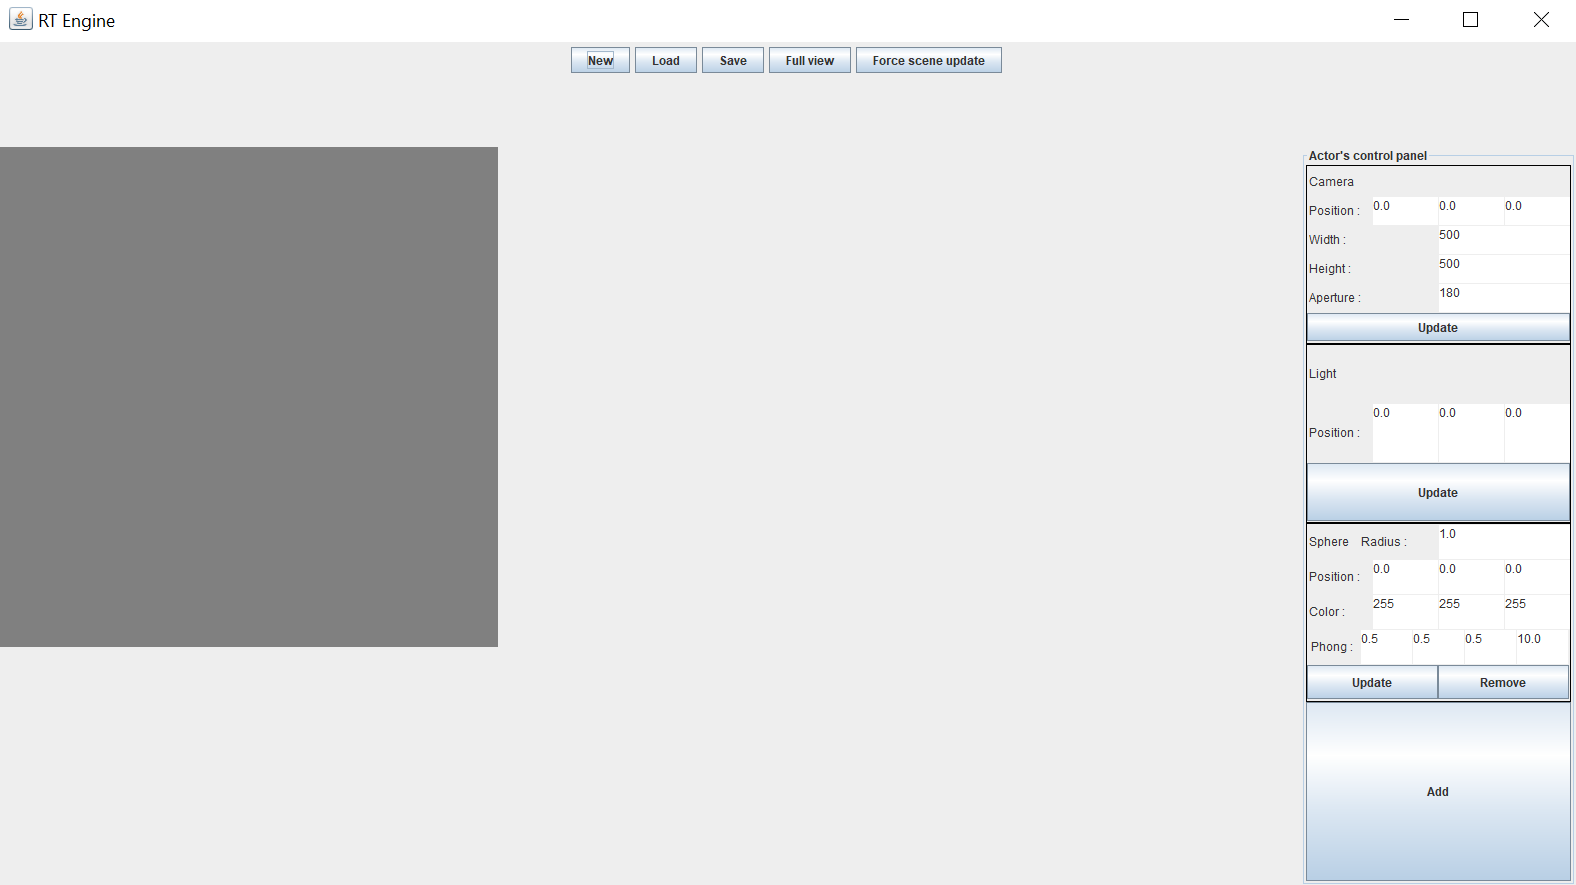
\includegraphics[width=0.9\textwidth]{./images/debut.png}
			\end{center}
			
		\paragraph{}
            Ici on a le possibilité de commencer a ajouter notre actor le sphere et en tant de fois qu'on veut  :
		        \begin{center}
	    	    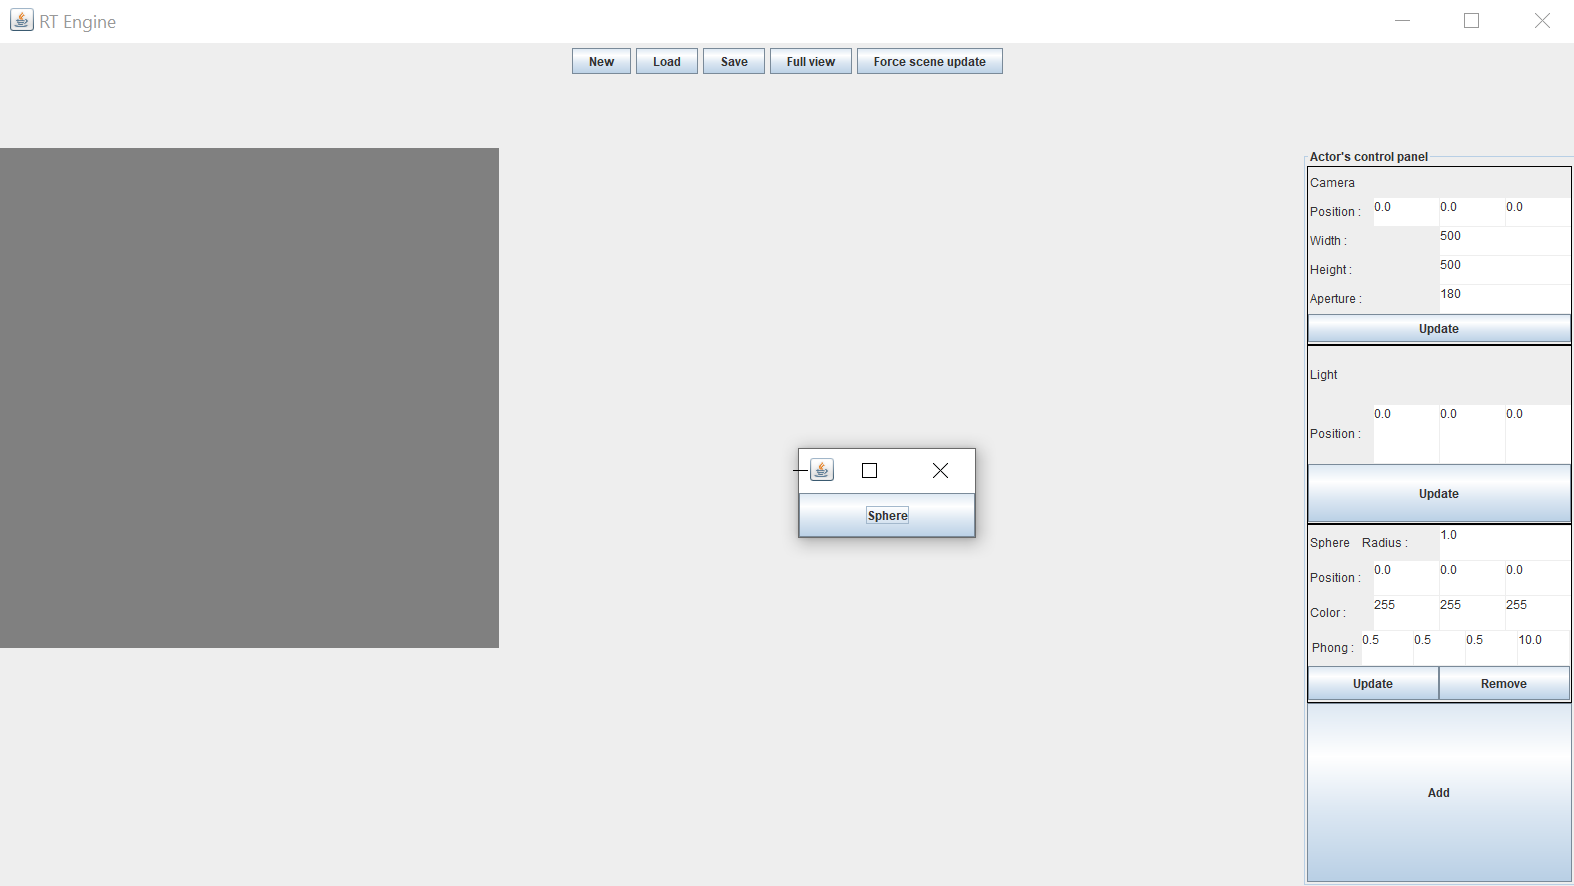
\includegraphics[width=0.9\textwidth]{./images/buttonsphere.png}
			    \end{center}
		\newpage
		\paragraph{}
            Par example ici on a ajouter trois spheres et il apparence sur notre tableau a droite comme on le voir ci-dessous :
		        \begin{center}
	           	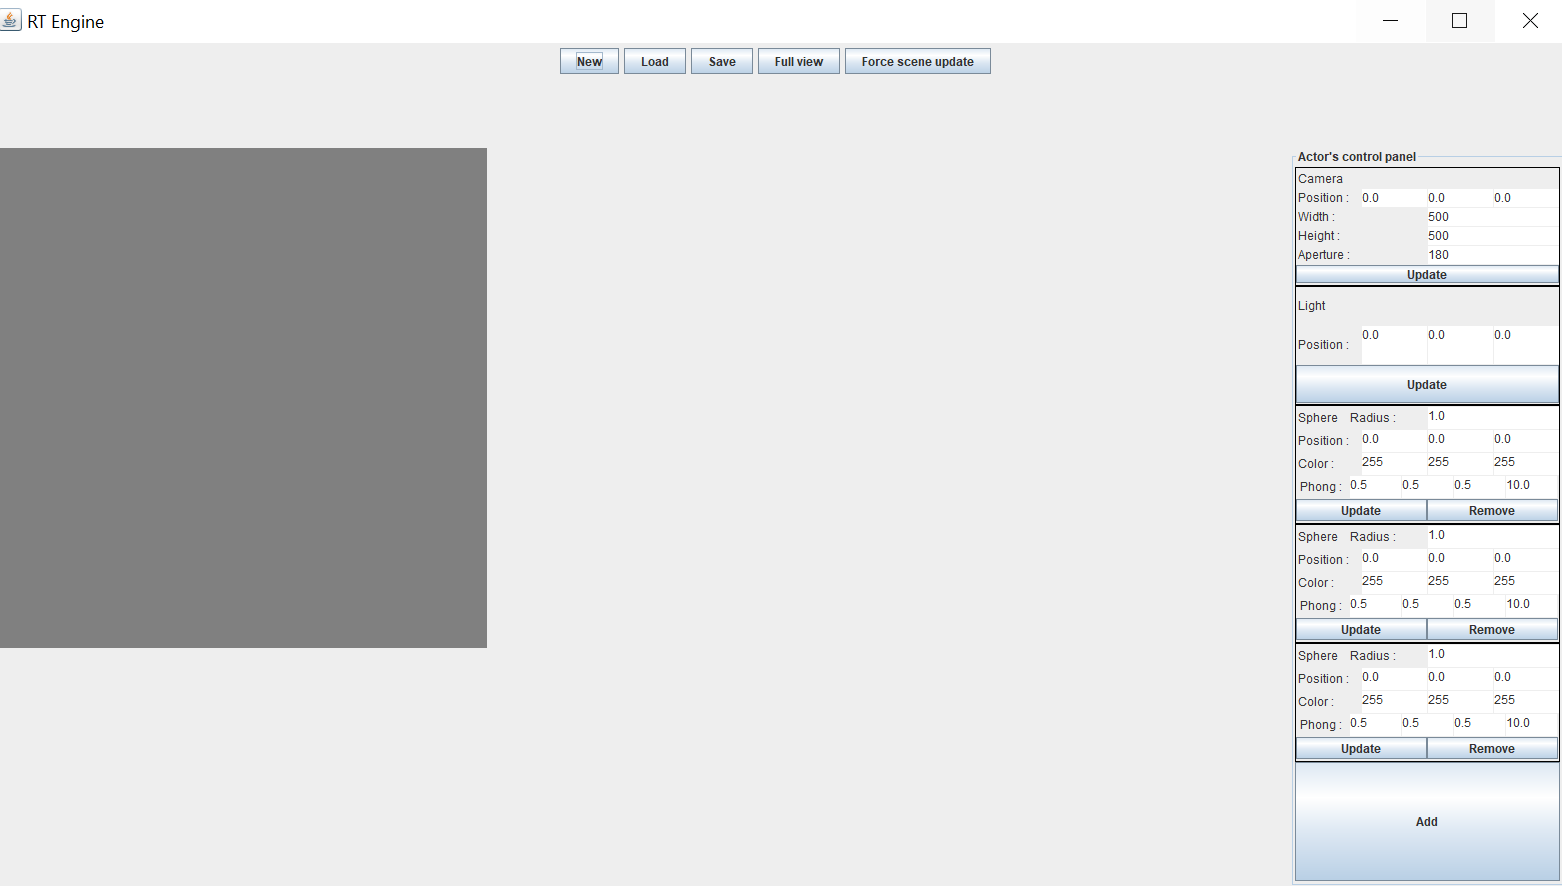
\includegraphics[width=0.9\textwidth]{./images/addsphere.png}
		    	\end{center}
			
		\paragraph{}
            pour cette etape on n'a la possibilté de changer la position de nos sphere ajouter précédemment ou on veux pour chaque sphere separement :
		        \begin{center}
	        	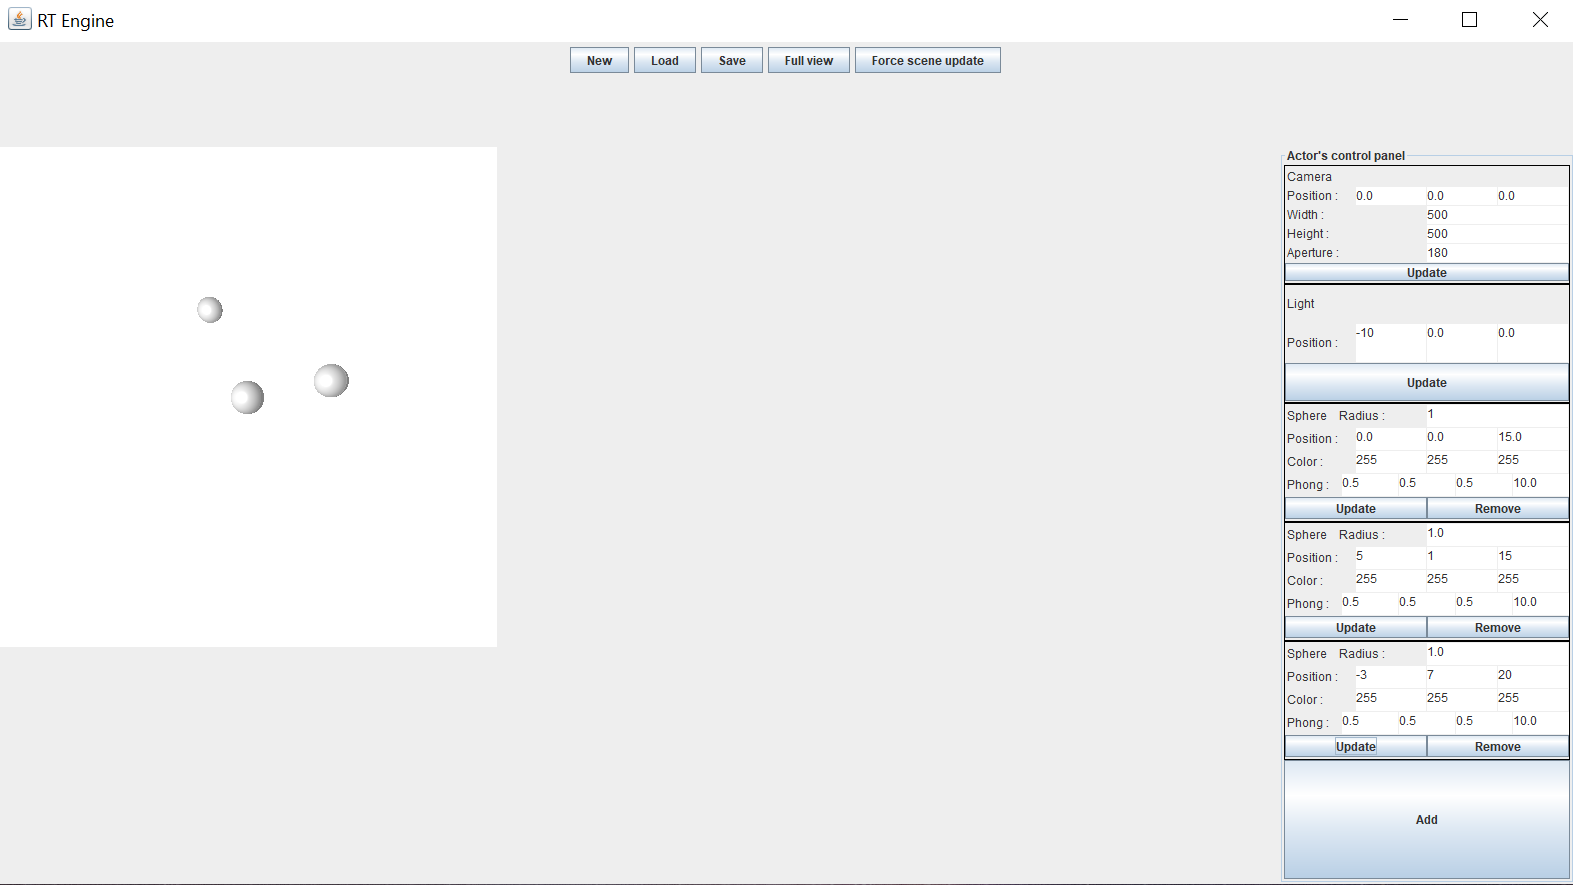
\includegraphics[width=0.9\textwidth]{./images/actorposition.png}
		    	\end{center}
		\newpage
		\paragraph{}
            ensuite en peux changer la coulour de chaque sphere tout seule comme on le veux :
		        \begin{center}
	           	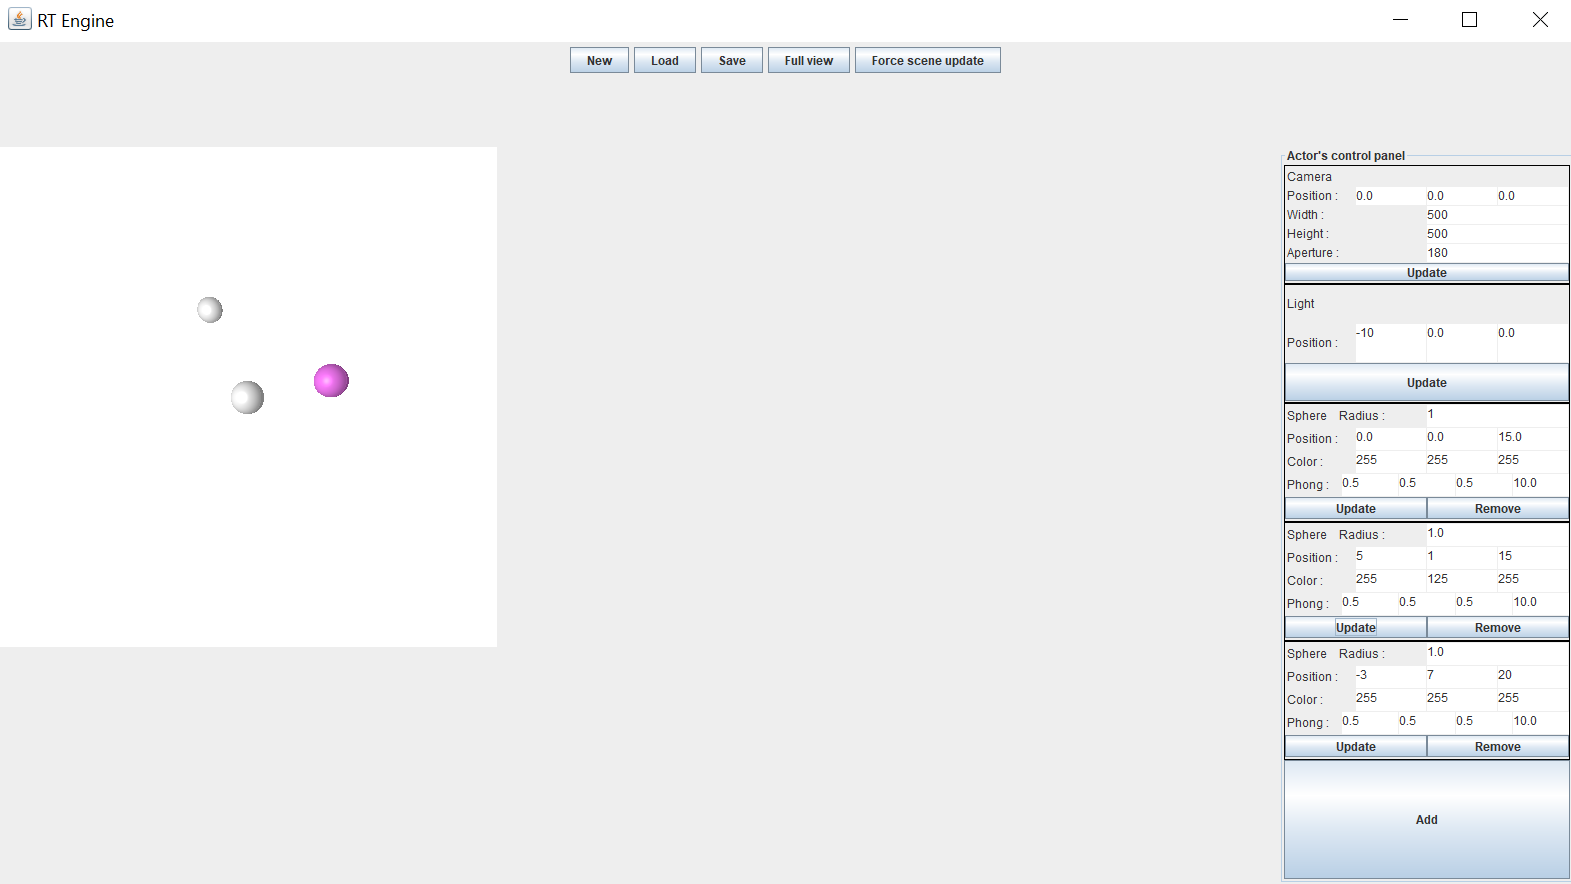
\includegraphics[width=0.9\textwidth]{./images/firstsphere.png}
		       	\end{center}
			
		\paragraph{}
            on fait la même chose pour le deuxième actor :
		        \begin{center}
	    	    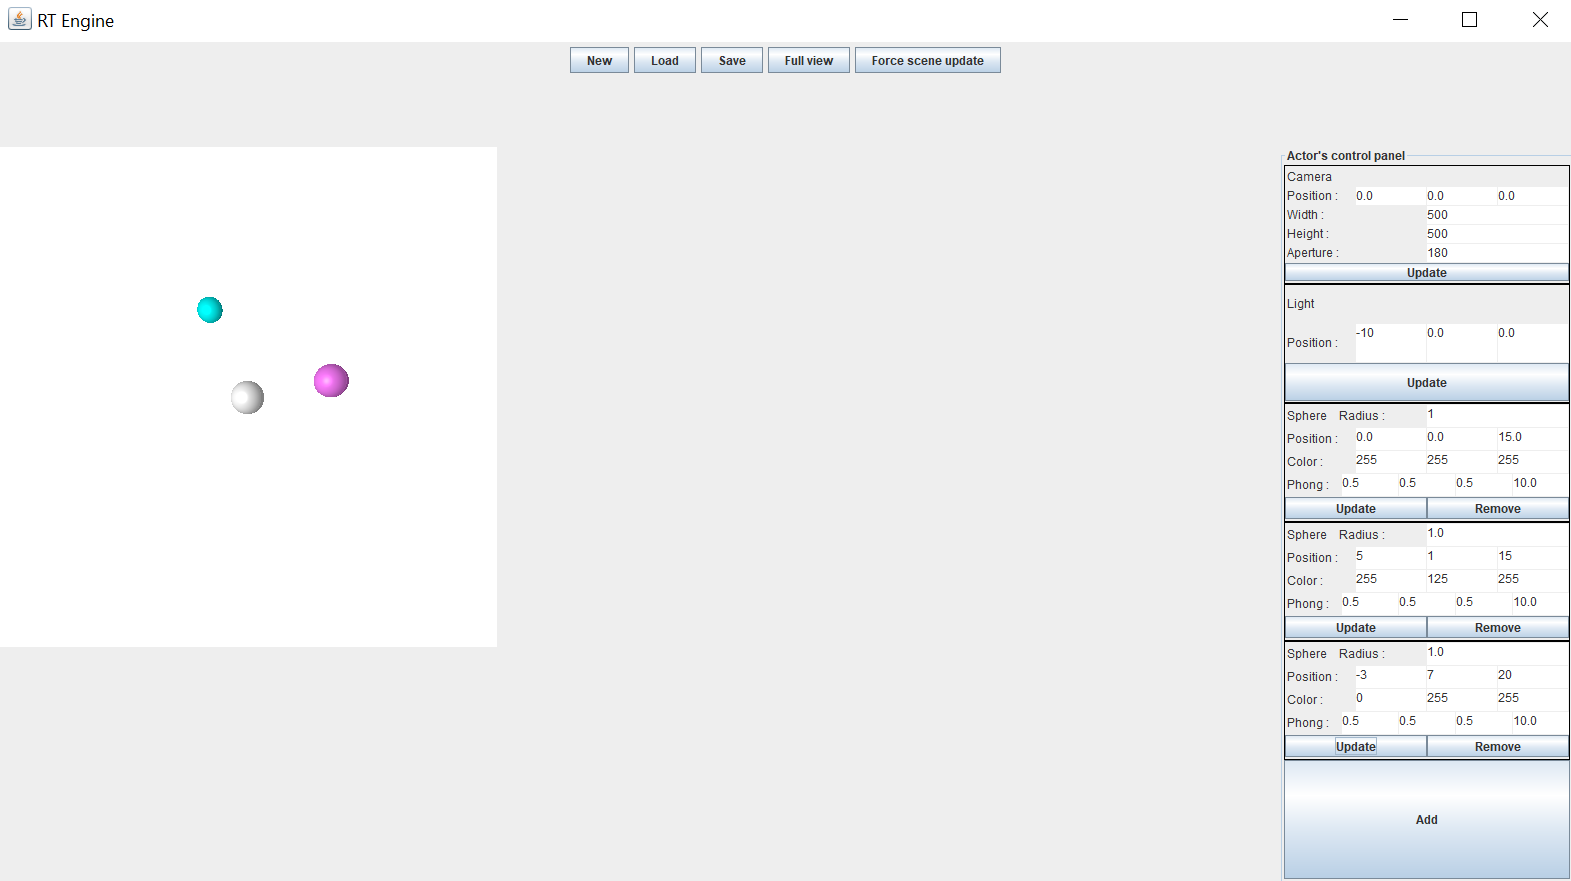
\includegraphics[width=0.9\textwidth]{./images/secondsphere.png}
			    \end{center}
		\newpage
		\paragraph{}
            et finalement pour notre dernier sphere la même chose on peux changer son coulour separement et comme on le veux aussi :
		        \begin{center}
	    	    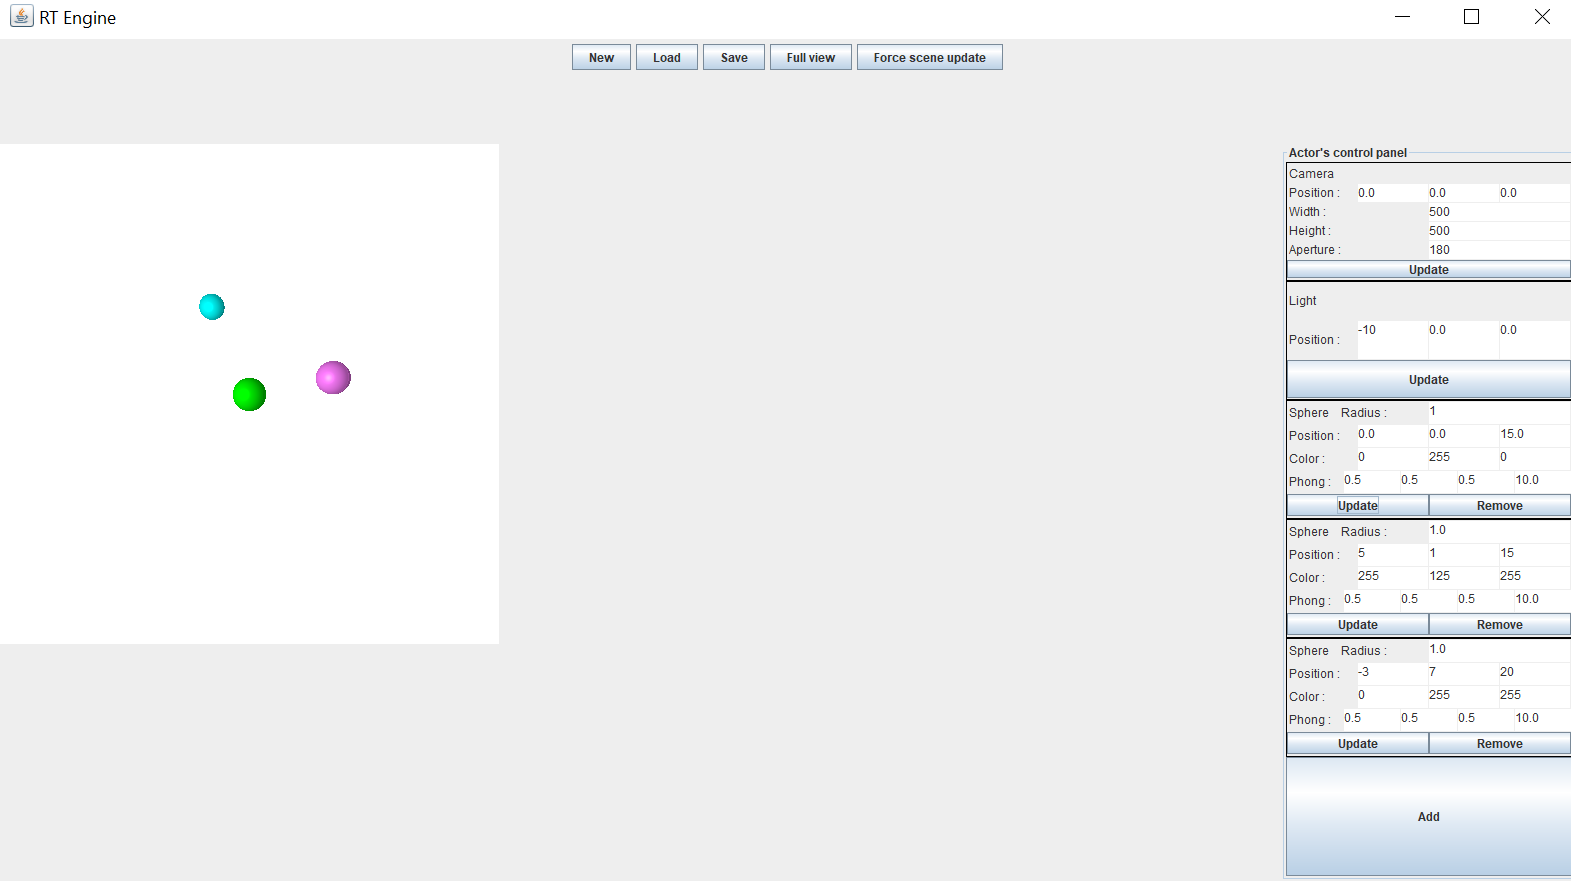
\includegraphics[width=0.9\textwidth]{./images/thirdsphere.png}
			    \end{center}
			
		\paragraph{}
            apres changer la coulour et la position on peut même changer la Raduis de notre sphere pour chaqu'un separemnt comme on le voir ci-dessous:
		        \begin{center}
	    	    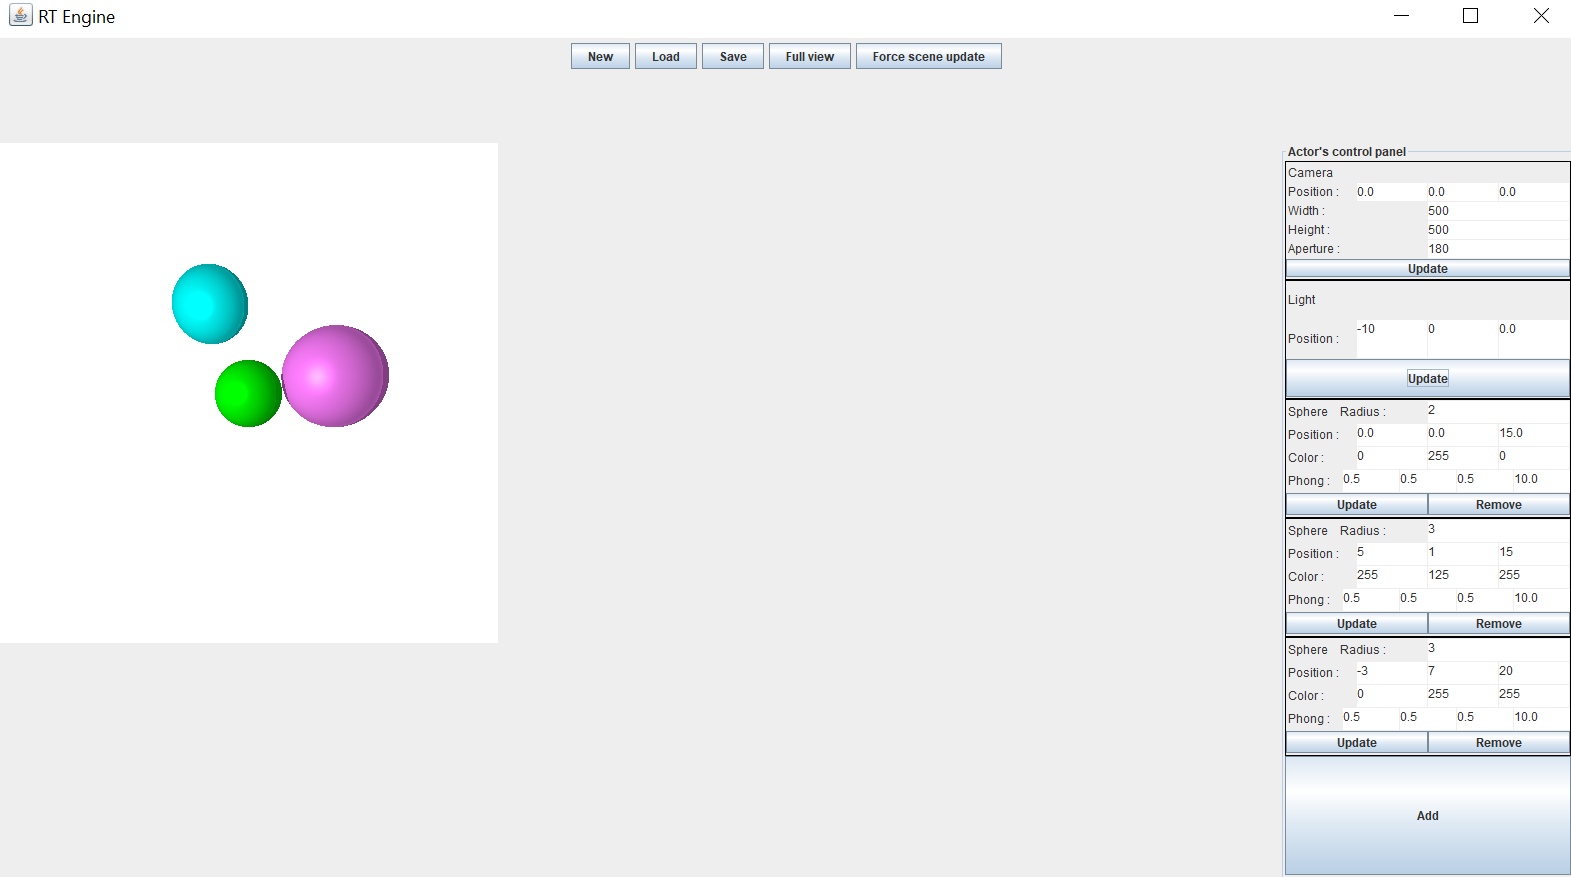
\includegraphics[width=0.9\textwidth]{./images/raduissphere.png}
	    	    \end{center}
        \newpage
	    \paragraph{}
            On peut même changer la position de la lumière comme ci-dessous : 
		        \begin{center}
	    	    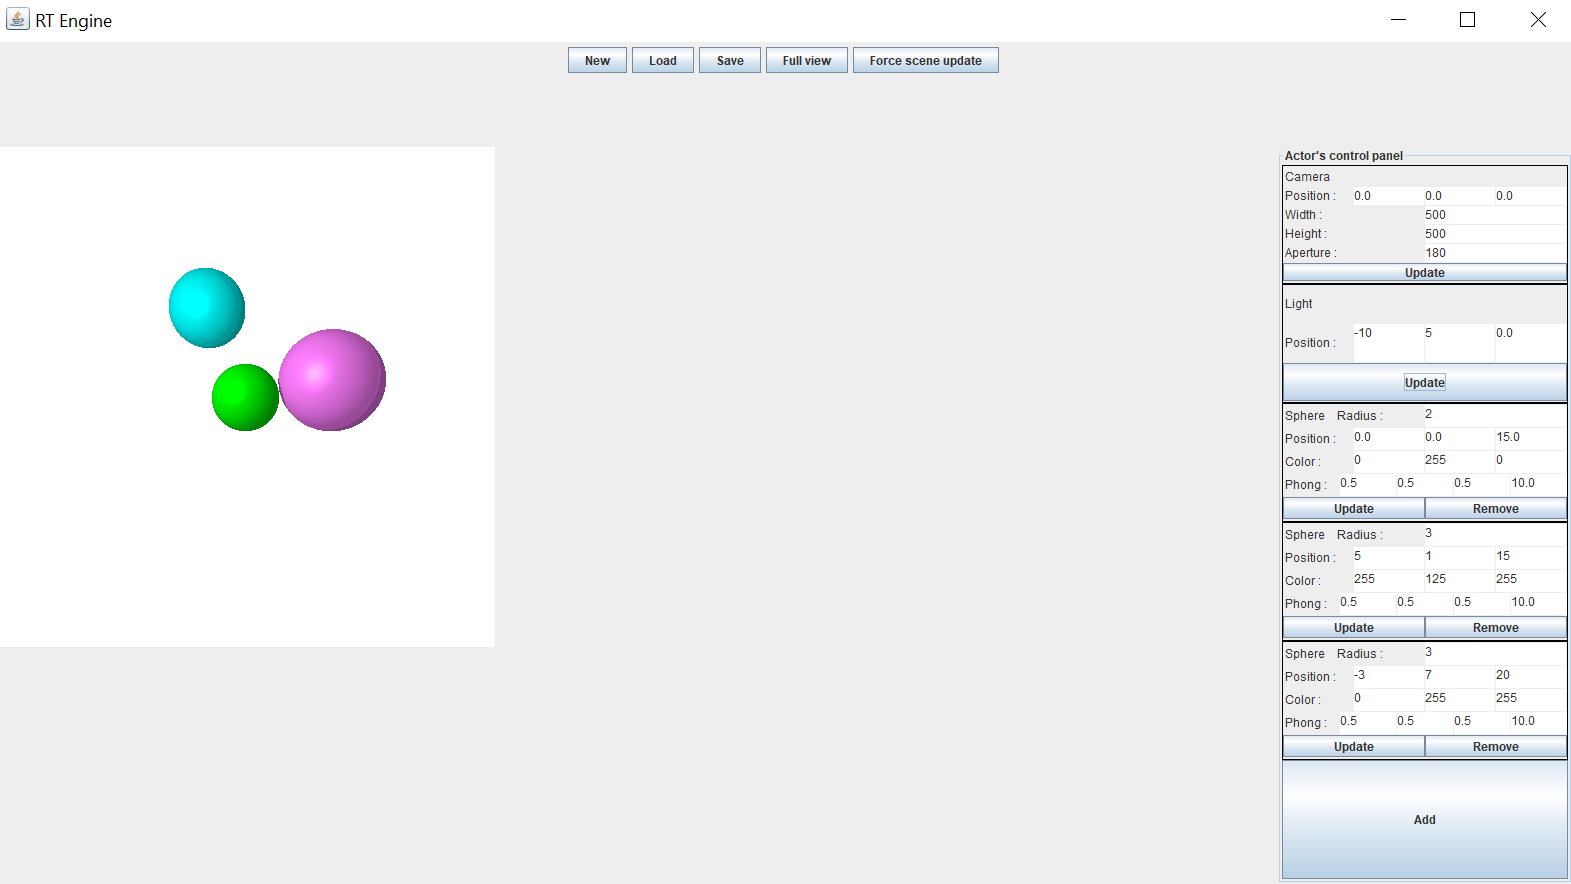
\includegraphics[width=0.9\textwidth]{./images/light.png}
			    \end{center}
			
		\paragraph{}
            maintenant après et a la fin on peut saugarder notre travaille juste on cliquant sur le button "save" et puis le donner un nom :
		        \begin{center}
	    	    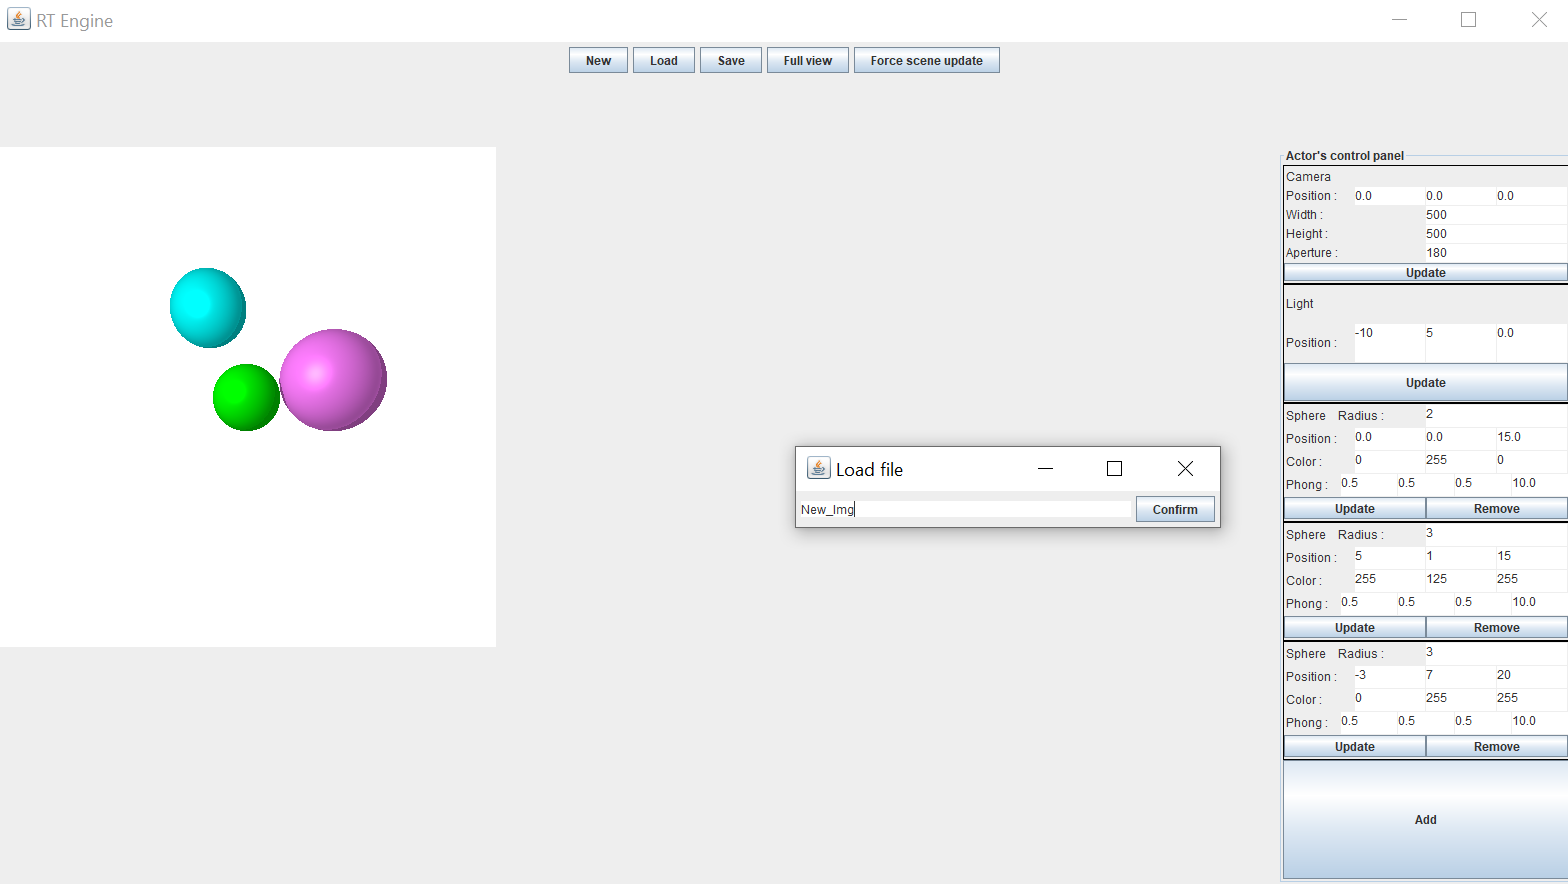
\includegraphics[width=0.9\textwidth]{./images/save.png}
			    \end{center}	
		\newpage
		\paragraph{}
            ainsi le button "full view" pour qu'on peut avoir notre image on grand image :
		        \begin{center}
	    	    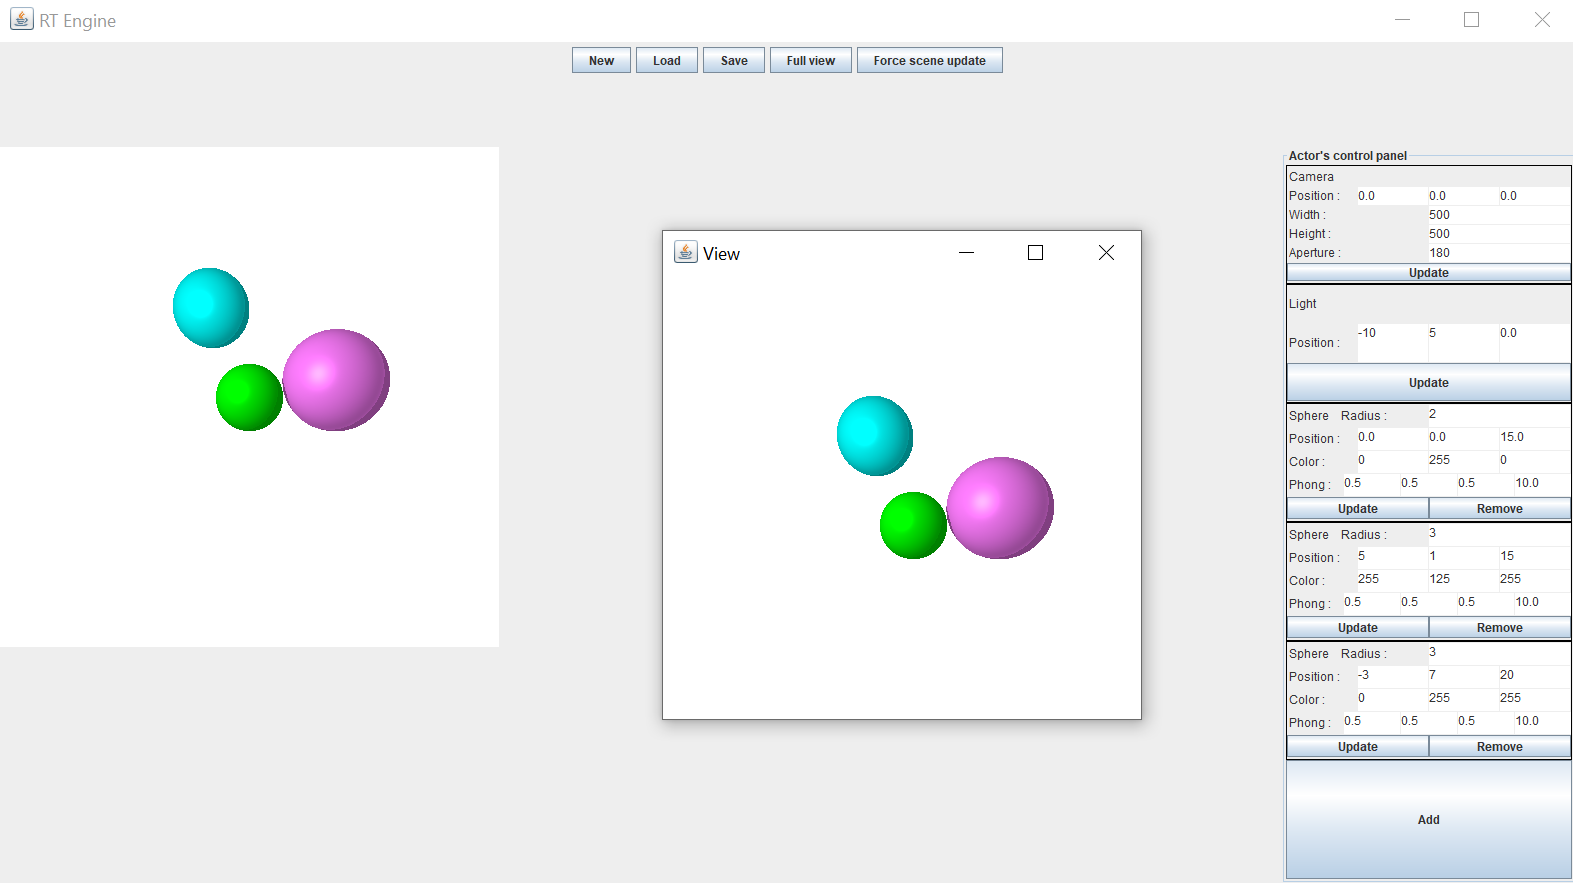
\includegraphics[width=0.9\textwidth]{./images/full_view.png}
			    \end{center}
			

		\subsection{Rendu final et manuel d'utilisation}
			\paragraph{Rendu final}
\begin{figure}[h]
			\begin{center}
	    	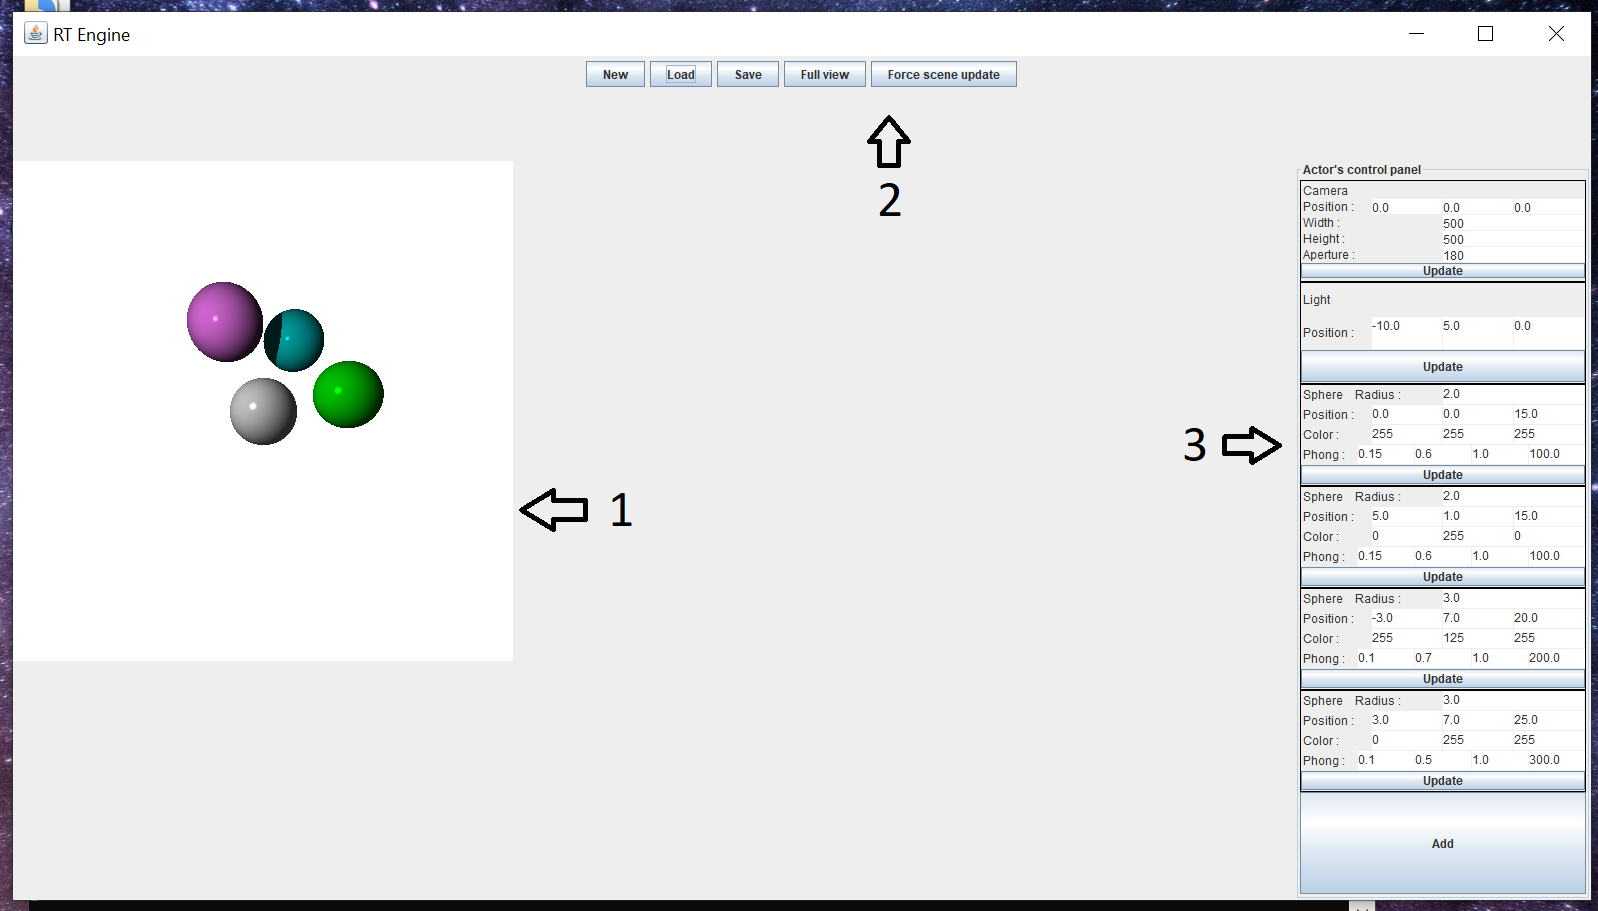
\includegraphics[width=0.9\textwidth]{./images/Capture.png}
			\end{center}
	\end{figure}
		  	\begin{enumerate}
		      \item La scène : dans cette partie on affiche notre scène en pré visualisation : L'image est plus petite ce qui permet une actualisation plus rapide a chaque modification.
		      \item Barre des options : C'est la que se situe les boutons de création de scène vide (New), de chargement de scène, si il y en a de sauvegardé (Load) , de sauvegarde de la scène actuelle  (Save), de visualisation a taille réelle de la scène avec possibilité de se déplacer (Full View) et enfin le bouton qui force la mise a jour de la scène en cas de bug (Force update)
		      \item Panneau des acteurs : Ce panneau permet la modification de la position de la caméra et des acteurs (sphère, lumière ...) ou la suppression d'acteurs. Ainsi que l'ajout d'acteurs dans la scène (bouton Add).
		  	\end{enumerate}
		  
		  	\paragraph{Manuel d'utilisation}
		  	Pour utiliser notre application il suffit de compiler grâce au script compiler (.bat pour windows, .sh pour linux) et de lancer la classe Main du package interface grâce au script run (.bat pour windows, .sh pour linux).
		  	
		  	Une fois l'application une scène vierge apparait, Vous pouvez soit ajouter un acteur grâce au bouton "Add" soit charger une scène grâce au bouton "Load" (un fichier "testParse.rt" existe déjà et peut être charger). Ensuite il suffit de compléter en ajoutant des acteurs et en modifier leurs valeurs.
		  	
		  	Une fois la scène créé il est possible de l'afficher en taille réelle et de se mouvoir dedans grâce en appuyant sur le bouton "Full view". Il est aussi possible de la sauvegarder grâce au bouton sauvegarder et en entrant un nom pour le fichier (sans l'extension.rt). 
		\subsection{Performances}
			\subsubsection{Benchmark}
			Pour savoir quels pourraient être les points d'optimisations du programme, il faut faire des test de performances. Ces test on été réalisé avec 3 configurations différentes :
			
			\begin{itemize}
				\item Ryzen 5-2600 (3.4GHz) + 24Go de RAM
				\item I3-6006U (2GHz) + 8Go de RAM
				\item I7-7600U (2.8GHz) + 16Go de RAM
			\end{itemize}
			
			Les test ont été faits sur les principales fonctions : "createRayList()" qui créé la liste des rayons nécessaires, "castRay()" qui lance les rayons, "refreshRay()" qui initialise les valeurs des rayons par défaut et "createImage()" qui créé l'image a partir des rayons.
			C'est cette image qui a été utilisé pour ces tests :
			\begin{center}
			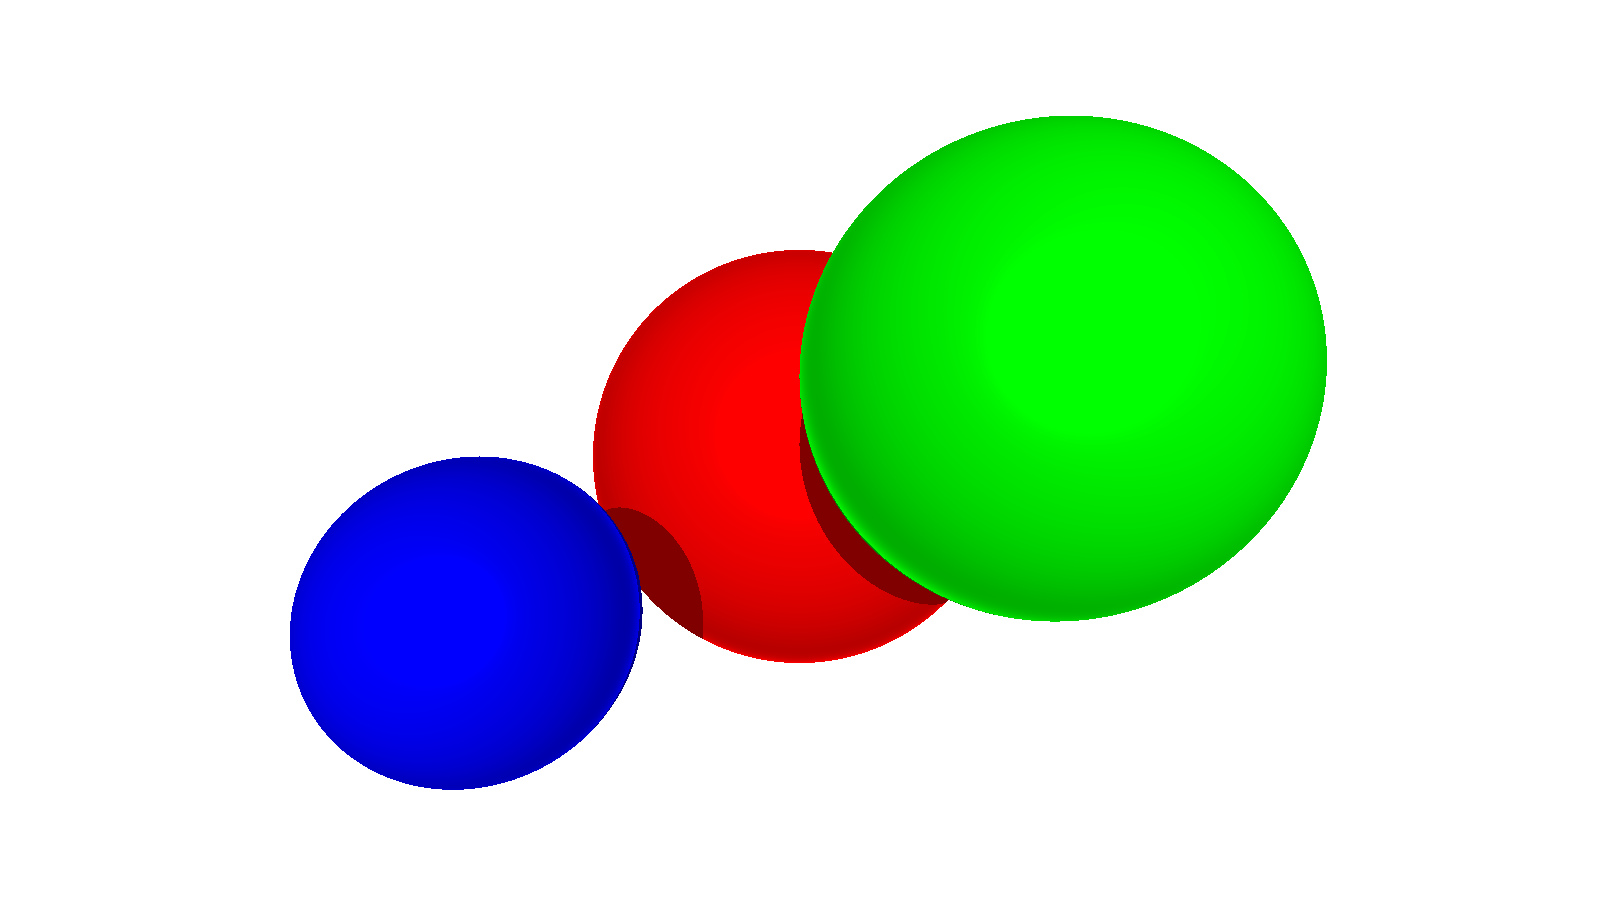
\includegraphics[scale=0.3]{./images/imgTest.png}
			\end{center}
			
			Les test ont été réalisé sur 2 définitions d'images différentes : 1600*900p et 1920*1080p. Ce qui nous donne les résultats suivant :
			\begin{center}
			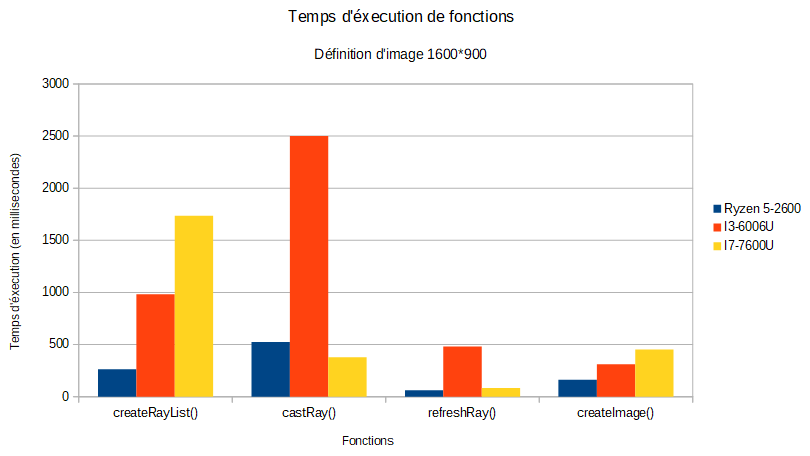
\includegraphics[scale=0.6]{./images/1600_900.png}\\
			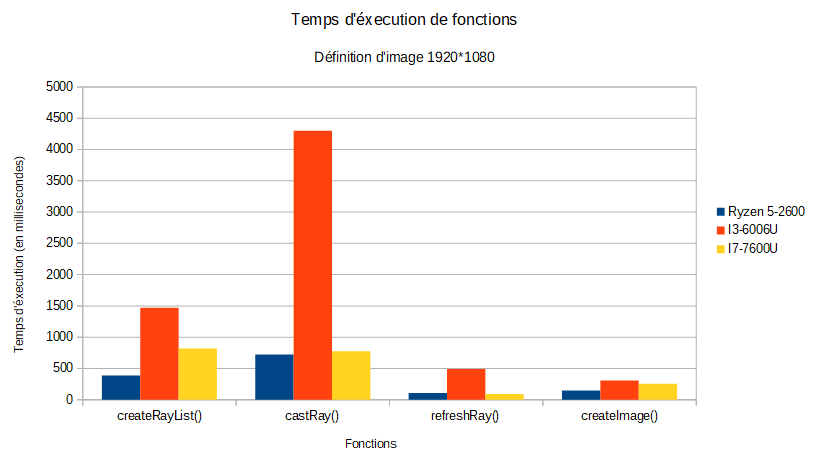
\includegraphics[scale=0.6]{./images/1920_1080.png}
			\end{center}
			On peut donc voir que la définition influe très peu la vitesse d'exécutions sur un processeur performant mais que moins le processeur est performant, plus le temps d'exécutions augmente pour les fonctions "createRayList()" et "castRay()". En revanche les fonctions "refreshRay()" et "createImage()" sont nettement moins influencé par la définition ou le processeur. Donc les fonctions "createRayList()" et "castRay()" sont prioritaires pour l'optimisation.
			
			\subsubsection{Optimisations possibles}
				\paragraph{Multi thread}
			Une des optimisations possible dans ce projet se situe sur le lancé de rayon, qui comme vu dans la partie performance, prend le plus de temps. Une piste d'optimisation serais d' utiliser le multi thread\footnote{En java un thread est un fil d'exécution, une suite d'instruction} qui consiste a faire plusieurs taches simultanément sur plusieurs thread au lieu d'un seul.
			
				\begin{figure}[!hbtp]
  					\begin{tikzpicture}
  						\node(mono) at (0,5) {\textit{Mono Thread}};
  						\node(t1_1) at (0,4) {Thread};
    					\node(task1_1) at (0,2) {Tache 1};
    					\node(task2_1) at (0,0) {Tache 2};
    					\node(multi) at (5,5) {\textit{Multi Thread}};
    					\node(t1) at (4,4) {Thread 1};
    					\node(t2) at (6,4) {Thread 2};
    					\node(task1) at (4,2) {Tache 1};
    					\node(task2) at (6,2) {Tache 2};
    					\node(start) at (9,4) {Début};
    					\node(end) at (9,0) {Fin};
    					\node(time) at (10,2) {Temps};
    					\draw[->] (t1_1) -- (task1_1);
    					\draw[->] (task1_1) -- (task2_1);
    					\draw[->] (t1) -- (task1);
    					\draw[->] (t2) -- (task2);
    					\draw[dashed] (start) -- (end);
  					\end{tikzpicture}
  					\caption{Comparaison simplifié entre mono et multi thread}
  					\label{fig:multithread}
				\end{figure}
			
				\begin{figure}[!hbtp]
  					\begin{tikzpicture}
  						\node(t1_1) at (0,4) {Thread};
    					\node(task1_1) at (0,2) {calcul intersection};
    					\node(actorhit) at (2,1) {Si acteur touché};
    					\node(task2_1) at (0,0) {calcul éclairage};
    					\draw[->] (t1_1) -- (task1_1);
    					\draw[->] (task1_1) -- (task2_1);
  					\end{tikzpicture}
  					\caption{Schéma du programme actuel}
  					\label{fig:currentschematic}
				\end{figure}		
			
				Pour cela nous avons plusieurs options d'utilisations, dans ces cas nous allons partir du principe que nous avons a disposition 2 thread (il s'agit du plus faible nombre de thread disponible pour le multi thread et aussi le plus faible nombre de thread disponible dans les configuration de PC actuelle) :
			
					\subparagraph{Option 1}
					La première option d'utilisation d'optimisation par multi thread serait logiquement de penser que pour le lancer de rayon nous avons le calcul des intersection avec les acteurs puis le calcul de l'éclairage. Donc sur un thread on calculerai le lancer de rayon et si un acteur est touché, de calculer l'éclairage de ce point (ou pixel) sur un autre thread pendant que le premier continu de calculer les intersections avec les acteurs.
					\begin{figure}[!hbtp]
  						\begin{tikzpicture}
    						\node(t1) at (0,4) {Thread 1};
    						\node(t2) at (5,4) {Thread 2};
    						\node(task1) at (0,0) {Calcul intersection};
    						\node(task2) at (5,0) {Calcul éclairage};
    						\node(actorhit)[rotate=40] at (2,2.3) {Si acteur touché};
    						\draw[->] (t1) -- (task1);
    						\draw[->] (t2) -- (task2);
    						\draw[->] (task1) -- (t2);
  						\end{tikzpicture}
  						\caption{Schéma de l'option 1}
  						\label{fig:option1}
					\end{figure}
			
					\subparagraph{Option 2}
					Le problème de la première option est qu'il y a très peu de cas où il y a autant de rayon qui touche un acteur que de rayon lancé. Dans la plupart des cas il y aura moins de point de l'image a éclairer que de rayon lancé. Donc une seconde option ou tous les rayons seraient calculés sur 2 thread est envisageable. On aurais juste a séparer la liste de rayons en 2 puis calculer chaque partie sur un thread différents puis de les éclairer :
			\begin{center}
					\begin{figure}[!hbtp]
  						\begin{tikzpicture}
    						\node(t1) at (0,4) {Thread 1};
    						\node(t2) at (5,4) {Thread 2};
    						\node(task1) at (0,2) {Calcul intersection};
    						\node(task2) at (0,0) {Calcul éclairage};
    						\node(task1_1) at (5,2) {Calcul intersection};
    						\node(task2_1) at (5,0) {Calcul éclairage};
    						\node(actorhit) at (2.5,1) {Si acteur touché};
    						\draw[->] (t1) -- (task1);
    						\draw[->] (task1) -- (task2);
    						\draw[->] (t2) -- (task1_1);
    						\draw[->] (task1_1) -- (task2_1);
  						\end{tikzpicture}
  						\caption{Schéma de l'option 2}
  						\label{fig:option2}
					\end{figure}
					\end{center}
				
					De cette manière on réduit théoriquement la durée de calcul par 2 puisqu'on effectue les calculs sur 2 rayons simultanément. En réalité ce ne sera pas forcément pas le cas car il n'y aura pas forcément autant d'intersection sur un thread que sur l'autre donc il y aura forcément une différence ce qui fera qu'on ne divisera pas exactement le temps mis par 2 et que cela dépendra de l'égalité d'intersection dans chaque thread.
				
				\paragraph{Factorisation du code}
				Il y a aussi beaucoup de problème d'optimisation au niveau de l'interface. En effet il y a beaucoup d'endroit avec des calculs inutiles dut a un manque de temps. Au lieu d'avoir par exemple une class abstraite qui permettrai de lancer une même fonction sur 3 class héritant de cette class abstraite , il y a 3 constructeurs différents, 3 attributs différents et 1 variable qui sert a utiliser le bon attribut :
			
				\lstinputlisting[language=Java, title={Code non optimisé/factorisé}, firstline=10, lastline=40]{../../engine/ui/UpdateButton.java}
			
				Dans ce cas on voit qu'avec une classe abstraite on pourrais avoir un seul constructeur et grandement alléger le nombre de calcul dans la fonction "actionPerformed". Ce qui donnerai quelques chose du genre :
			
				\begin{lstlisting}[language=Java, title="Idée de factorisation"]
private abstractPanel panel
			
public UpdateButton(String title, abstractPanel panel){
	super(title);
	this.panel = panel;
}
			
public void actionPerformed(ActionEvent e){
	this.panel.setValue();
}
			\end{lstlisting}
		
			Il y a aussi d'autres problèmes d'optimisation sur l'interface avec des panels qui sont totalement recalculé a chaque actualisation de l'application. Par exemple le panel "ActorControl" est totalement recalculé a chaque acteur ajouté.
		
			\paragraph{Visualisation de la scène}
			Comme vu précédemment, la generation de l'image prend plus ou moins 1 seconde (cela dépend bien sur du processeur). Donc lorsqu'on affiche la scène avec la possibilité de se déplacer dessus, Chaque mouvement recalcule la scène. Pour limiter le nombre de calcul une possibilité serais de stocker l'image généré et ainsi a chaque mouvement de la caméra vérifier si l'image correspondante a déjà été calculé ou non. Si elle a été calculé alors on la récupère et on l'affiche, sinon on la calcul on l'affiche et on la stock pour plus tard.
			Il y a tout de même un gros inconvénient a cette solution. Si le nombre d'image stocké deviens trop important on risque de surcharger la mémoire RAM en plus de possiblement atteindre un nombre de calcul aussi important que si on devais recalculer l'image. Sans parler du nombre d'image possiblement générer si on y ajoute tous les rotations de caméra possible.
			Cette solution est donc possible pour un nombre modéré d'images, mais dans un cas ou l'utilisateur veut se promener dans la scène cette solution n'est pas adapté.
		
		\newpage
		\section{Conclusion}
	
		\subsection{État des objectifs}
		
	\paragraph{}L'objectif principal de ce projet est de réaliser une application en langage java en groupe permettant ainsi d'évoluer en travail d'équipe et de réaliser un moteur de rendu 3D.
	
		\subsubsection{Objectifs atteints}
		
	\paragraph{} Les objectifs atteints  pour réaliser ce projet sont l'implémentation de la réflexion et de la réfraction suivit de l'ombrage de Phong sont utilisables. L'implémentation d'un parse ainsi que la sauvegarde des éléments de l'image sont eux bien pris en charge. De plus un interface graphique avec des boutons interactifs sont eux aussi mis à la disposition de l'utilisateur. Seul la sauvegarde du fichier est quant a lui partiellement atteint l'image enregistrer n'utilise pas la totalité d'un fichier pov. 
	
		\subsubsection{Objectifs non atteints}
		
	\paragraph{}Les objectifs non atteints sont l'ajout d'autre formes ainsi que le pivotement de la camera. L'un des objectifs étaient de pouvoir enregistrer nos images en pov, chose qui fut partiellement réussi car nous pouvons sauvegarder notre contenu d'image mais sans utiliser toutes les caractéristiques du pov.
		\subsection{Améliorations possibles}
		
	\textit{Des améliorations sont possibles à réaliser avec la factorisation de code ou avec la mise en place d'autre fonction permettant d'alléger les calculs ou de simplifier la réalisation de certaine tache. }
		\subsubsection{Contenu disponible}
		
	\paragraph{} Nous avons un contenu limité avec l'affichage d'une forme unique qui est la sphère. D'autres formes auraient pu être implémenté tels que des cônes, des cylindres ou des cubes.
	
		\subsubsection{Fonctionnalités}
	
	\paragraph{}De nombreuses fonctionnalités aurait pu être ajouté au projet tels que la rotation de la caméra et des acteurs, la réflection des objets entre eux ou l'ajout de transparence des objets (pour recrée des matière comme le metal avec une multiple réflection ou du verre pour la transparence.
			
\end{document}